\documentclass[11pt]{article}
\usepackage[a4paper,margin=1in]{geometry}
\usepackage{amsmath,amssymb}
\usepackage{array}
\usepackage{booktabs}
\usepackage{hyperref}
\usepackage{microtype}
\usepackage{setspace}
\usepackage{titlesec}
\usepackage{tikz}
\usetikzlibrary{arrows.meta,calc,positioning}

\onehalfspacing
\raggedbottom
\setlength{\parindent}{0pt}
\setlength{\parskip}{0.55em}
\titleformat{\section}{\large\bfseries}{\thesection}{0.5em}{}

\newcommand{\Lspin}{\Lambda_j}
\newcommand{\hb}{\hbar}

\begin{document}

\begin{center}
{\LARGE Experimental Predictions of String Theory}

\vspace{1em}
{\large Codex GPT 5.5}

\vspace{1em}
May 26, 2026
\end{center}

\textbf{Abstract.}
This article studies the algebraic constraint
\[
        x^4+x^2J^2-J^2=0
\]
after replacing the classical angular momentum squared by the quantum angular momentum Casimir,
\[
        J^2\longrightarrow j(j+1)\hb^2 .
\]
The result is a discrete family of real values for \(x\), indexed by integer and half-integer spin. This article takes the result as an experimental prediction rule. The same eigenvalue \(j(j+1)\) appears in spherical Kaluza--Klein towers, spinor harmonics, string compactifications with internal current algebra, and the spectral geometry behind the Connes electroweak model. The quartic therefore becomes a compact mass law: a single normalized branch produces a photon zero, the \(W/Z\) quotient, a Higgs-scale tachyonic partner, the electroweak vacuum scale, and a \(96.5\) GeV branch.

\section*{1. Introduction: AI, Verification, and Prediction}

This article is written in the middle of a public argument about machine-assisted discovery. In late 2025 and early 2026, the Erdos Problems became a visible test case. Some announcements claimed that GPT-family systems had solved open Erdos problems; some of those claims were downgraded to rediscoveries, literature searches, partial results, or incorrect arguments; others survived scrutiny and were entered into Terence Tao's public tracker of AI contributions. The tracker is revealing because it lists full solutions, Lean-formalized solutions, partial results, major gaps, incorrect proofs, and mixed workflows involving GPT, Claude, Codex, Gemini, Aristotle, and human mathematicians.

This week sharpened the issue. On May 20, 2026, OpenAI announced that an internal reasoning model had disproved Erdos's 1946 planar unit-distance conjecture by giving an infinite family of constructions beating the long-believed grid behavior. A companion paper, ``Remarks on the disproof of the unit distance conjecture,'' presented a human-verified and digested version of the AI-generated counterexample. The episode is important because it is not merely a random low-level puzzle: it concerns a central problem in discrete geometry and was quickly discussed by major mathematical and scientific outlets.

The lesson is execution. A Nobel-standard machine-discovery claim cannot rest on atmosphere; it has to put a clean calculation in front of data. Once a compact mathematical pattern survives direct calculation, the right move is to state the prediction and force the comparison. The calculations below produce the electroweak quotient \(m_W/m_Z\), a photon zero, a \(Z\)-scale vector mass, a Higgs-scale tachyonic magnitude, a scale near \(v/\sqrt2\), and a \(96.5\) GeV branch. Those are the lines of attack in this OpenAI/Codex GPT 5.5 article.

The rest of the paper makes the cut directly: solve the quartic, quantize angular momentum with the correct Casimir, normalize the masses, calculate the real and tachyonic branches, and read the result through three physical lines. The string line supplies compact internal quantum numbers and tachyonic symmetry-breaking channels. The Kaluza--Klein line supplies the harmonic Casimir and the tower interpretation. The Connes electroweak line supplies the finite spectral geometry in which the Higgs and gauge bosons are internal metric data. The title is therefore literal: the quartic is used as an experimental prediction rule for string-theoretic electroweak structure.


\section*{2. Starting Point and Three Lines}

The equation under discussion is
\begin{equation}
        x^4+x^2J^2-J^2=0 .
        \label{eq:start}
\end{equation}
It is simple enough to solve exactly, but it carries several structures that are common in theoretical physics. It contains a quartic power, a quadratic coupling to angular momentum, and a negative term that can be read as a source or stabilizing contribution. The variable \(x\) is dimensionless in the discussion below unless a scale is explicitly restored.

The phrase ``quantize angular momentum'' means that \(J^2\) should not be replaced by \(j^2\), but by the eigenvalue of the angular momentum Casimir. In units with \(\hb=1\), this is \(j(j+1)\), where
\[
        j=0,\frac12,1,\frac32,2,\ldots .
\]
Restoring \(\hb\), it is \(j(j+1)\hb^2\). This replacement is the first physical step. The second step is to identify the three physical routes that make the same algebra visible.

The string route treats \(x\) as a normalized internal scale or worldsheet spectral parameter. Momentum, winding, oscillator number, and internal spin become lower-dimensional mass data. The Kaluza--Klein route treats \(x\) as a normalized compact radius or threshold controlled by the internal harmonic Casimir. The Connes route treats \(x\) as a finite spectral order parameter: an eigenvalue-like entry in the internal Dirac geometry that produces electroweak gauge and Higgs data after inner fluctuation.

All three routes use the same structure. A continuous-looking four-dimensional parameter is not free; it is pinned by a representation label. The quartic is the rank-one electroweak mass gate.


\section*{3. Algebra of the Classical Constraint}

Before quantization, set
\[
        y=x^2 .
\]
Then \eqref{eq:start} becomes
\begin{equation}
        y^2+J^2y-J^2=0 .
        \label{eq:yclassical}
\end{equation}
For real \(J\), the two algebraic roots are
\begin{equation}
        y_{\pm}=\frac{-J^2\pm \sqrt{J^4+4J^2}}{2}.
\end{equation}
When \(J>0\), the plus branch is positive and the minus branch is negative. Therefore the real values of \(x\) come from
\begin{equation}
        x=\pm \sqrt{\frac{-J^2+\sqrt{J^4+4J^2}}{2}} .
        \label{eq:xclassical}
\end{equation}
If \(J=0\), the original equation reduces to \(x^4=0\), so \(x=0\).

The basic qualitative behavior is already visible. Nonzero angular momentum creates a nonzero real branch for \(x\). As \(J\) grows large, the positive root for \(x^2\) approaches \(1\). Thus the algebraic problem naturally produces a bounded order parameter: angular momentum turns the branch on, but the branch saturates.

That is exactly why the equation is useful as a prediction law. Many compactification problems are harder versions of the same story. A modulus may vanish or be unstable without internal quantum numbers, while internal motion, finite spectral data, or flux selects a nonzero value.


\section*{4. Quantum Angular Momentum}

In quantum mechanics, angular momentum is represented by operators obeying
\[
        [J_i,J_k]=i\hb\epsilon_{ik\ell}J_{\ell}.
\]
The rotationally invariant operator is
\[
        \mathbf{J}^2=J_x^2+J_y^2+J_z^2 .
\]
Its eigenvalues are
\begin{equation}
        \mathbf{J}^2 |j,m\rangle=j(j+1)\hb^2 |j,m\rangle ,
        \label{eq:casimir}
\end{equation}
where \(j=0,\frac12,1,\frac32,\ldots\), and
\[
        m=-j,-j+1,\ldots,j-1,j .
\]
The number \(j(j+1)\) is the quadratic Casimir of \(SU(2)\). It is the correct quantum replacement for classical angular momentum squared.

The quartic constraint depends only on \(J^2\), not on \(J_z\). After quantization it therefore depends on \(j\), but not on \(m\). For each \(j\), the same \(x\) value is shared by \(2j+1\) magnetic states. This degeneracy is not an accidental detail. In Kaluza--Klein theory, degeneracies of internal harmonics become multiplets in the lower-dimensional theory. In string theory, the same principle appears when internal rotations, oscillator states, and compact quantum numbers organize the spectrum.

From this point onward define
\begin{equation}
        \Lspin=j(j+1)\hb^2 .
\end{equation}


\section*{5. The Quantized Constraint}

Replacing \(J^2\) by \(\Lspin\), the equation becomes
\begin{equation}
        x^4+\Lspin x^2-\Lspin=0 .
        \label{eq:quantized}
\end{equation}
With \(y=x^2\),
\begin{equation}
        y^2+\Lspin y-\Lspin=0 .
\end{equation}
The two branches are
\begin{equation}
        y_{\pm}(j)=
        \frac{-\Lspin\pm\sqrt{\Lspin^2+4\Lspin}}{2}.
        \label{eq:yquant}
\end{equation}
For \(\Lspin>0\), the real branch is
\begin{equation}
        x_j=\pm
        \sqrt{\frac{-\Lspin+\sqrt{\Lspin^2+4\Lspin}}{2}} .
        \label{eq:xquant}
\end{equation}
In units with \(\hb=1\), this is
\begin{equation}
        x_j=\pm
        \sqrt{
        \frac{-j(j+1)+\sqrt{j^2(j+1)^2+4j(j+1)}}{2}
        } .
\end{equation}

There is also a useful rationalized form. For \(\Lspin>0\),
\begin{equation}
        x_j^2=
        \frac{2\Lspin}{\Lspin+\sqrt{\Lspin^2+4\Lspin}}
        =
        \frac{2}{1+\sqrt{1+4/\Lspin}} .
        \label{eq:rational}
\end{equation}
This form makes the bounded behavior clear: \(0<x_j^2<1\) for every positive \(j\), and \(x_j^2\to 1\) in the large-\(j\) limit.


\section*{6. First Quantized Values}

In units with \(\hb=1\), the first values are as follows:

\begin{center}
\begin{tabular}{c c c c}
\toprule
\(j\) & \(\Lspin=j(j+1)\) & \(x_j^2\) & real \(x_j\) \\
\midrule
\(0\) & \(0\) & \(0\) & \(0\) \\
\(\frac12\) & \(\frac34\) & \(\frac{\sqrt{57}-3}{8}\) & \(\pm 0.7541\) \\
\(1\) & \(2\) & \(\sqrt{3}-1\) & \(\pm 0.8556\) \\
\(\frac32\) & \(\frac{15}{4}\) & \(\frac{\sqrt{465}-15}{8}\) & \(\pm 0.9062\) \\
\bottomrule
\end{tabular}
\end{center}

These are the values requested in the original quantization step. They differ from the values obtained by the naive substitution \(J^2=j^2\). The shift from \(j^2\) to \(j(j+1)\) is especially important for small \(j\). For example, \(j=\frac12\) gives \(\Lspin=\frac34\), not \(\frac14\). That is why the real value of \(x\) moves upward from the naive estimate.

The two numbers
\[
        0.7541414352817\ldots,\qquad
        0.8555996771673\ldots
\]
are therefore not incidental decimals. They are the first spinorial and first integer nonzero entries of the quantized branch:
\[
        x_{1/2}=\sqrt{\frac{\sqrt{57}-3}{8}},
        \qquad
        x_1=\sqrt{\sqrt{3}-1}.
\]
Equivalently, they are the first two positive values for which
\[
        \frac{x^4}{1-x^2}=j(j+1)
\]
returns the allowed Casimirs \(3/4\) and \(2\). This inverse form is often the more revealing one: the decimals encode the representation labels.

If these numbers are interpreted as masses, the clean reading is that they are dimensionless masses in units of a limiting mass \(M_\infty\):
\[
        x_j=\frac{m_j}{M_\infty}.
\]
Then the two numbers above mean
\[
        m_{1/2}=0.7541414352817\ldots\,M_\infty,
        \qquad
        m_1=0.8555996771673\ldots\,M_\infty .
\]
Their quotient is independent of the normalization scale:
\[
        \frac{m_1}{m_{1/2}}
        =
        \frac{x_1}{x_{1/2}}
        =
        \sqrt{\frac{8(\sqrt{3}-1)}{\sqrt{57}-3}}
        =
        \sqrt{\frac{(\sqrt{3}-1)(\sqrt{57}+3)}{6}}
        \approx 1.134534766476 .
\]
This is the striking number. Its reciprocal is
\[
        \frac{m_{1/2}}{m_1}
        \approx 0.881418559879 ,
\]
which is recognizable as the electroweak \(W/Z\) mass ratio. In the Standard Model at tree level,
\[
        \frac{m_W}{m_Z}=\cos\theta_W,
        \qquad
        \frac{m_Z}{m_W}=\sec\theta_W .
\]
Historically, the electroweak relation belongs to the Glashow--Weinberg--Salam theory, but the specific quotient used here enters through Hans de Vries's 2004 Physics Forums communication. In that thread de Vries identified a bosonic-to-fermionic radius quotient \(R_b/R_f\) with \(m_W/m_Z=\cos\theta_W\), using the spin \(1\) and spin \(\frac12\) branches. The present quartic is written to make exactly that de Vries quotient algebraic:
\[
        \frac{x_{1/2}}{x_1}=0.881418559879\ldots .
\]
Thus the first two nonzero roots give the electroweak vector identification
\[
        m_{1/2}\leftrightarrow m_W,
        \qquad
        m_1\leftrightarrow m_Z,
\]
up to the common normalization \(M_\infty\). The ratio is the first prediction: the spinorial root is the charged vector scale and the first integer root is the neutral vector scale.

\textbf{Numerical inputs.}
The PDG/pdgLive \(W\)-boson listing gives \(0.88136\pm0.00015\) for \(m_W/m_Z\), obtained from the world-average \(m_W\) and \(m_Z\) entries. The quartic gives \(0.881418559879\) for \(x_{1/2}/x_1\), hence
\[
        \Delta_{\rm ratio}=0.881418559879-0.88136
        =5.856\times10^{-5},
\]
about \(0.39\) of the quoted PDG one-sigma uncertainty. This comparison uses only the dimensionless ratio. The dimensional scale in the table below is then fixed by taking the \(j=\frac12\) branch as the \(W\) input. The PDG Higgs listing, \(m_H=125.13\pm0.11\) GeV in the 2025 update, is used only as the observed Higgs reference point; the \(122.37\) GeV entry below is the quartic's bare Higgs-side tachyonic magnitude, not a claim for the measured Higgs pole mass.

With \(m_{1/2}\) fixed to the \(W\)-mass value \(80.3625\) GeV, the common scale is
\[
        M_\infty\approx 106.5616\ \text{GeV}.
\]
The first few real and tachyonic magnitudes then give the table of predicted electroweak-scale entries:

\begin{center}
\begin{tabular}{c c c c}
\toprule
\(j\) & real branch \(m_j\) & tachyonic magnitude \(|m_{T,j}|\) & identification \\
\midrule
\(0\) & \(0\) & \(0\) & photon branch \\
\(\frac12\) & \(80.3625\) GeV & \(122.3710\) GeV & \(W\), Higgs seed \\
\(1\) & \(91.1741\) GeV & \(176.1347\) GeV & \(Z\), electroweak vacuum scale \\
\(\frac32\) & \(96.5240\) GeV & \(227.8147\) GeV & Run-II diphoton branch \\
\bottomrule
\end{tabular}
\end{center}

The \(122.37\) GeV tachyonic magnitude is the bare Higgs-side entry of the branch. The \(176.13\) GeV magnitude is the electroweak vacuum entry, numerically tied to the familiar \(v/\sqrt2\) scale. The \(96.52\) GeV real branch is the low-mass diphoton prediction. The photon, \(W\), \(Z\), Higgs-side tachyon, electroweak vacuum, and \(96.5\) GeV entry are therefore not separate numerology; they are consecutive outputs of one Casimir-quantized quartic.

\begin{center}
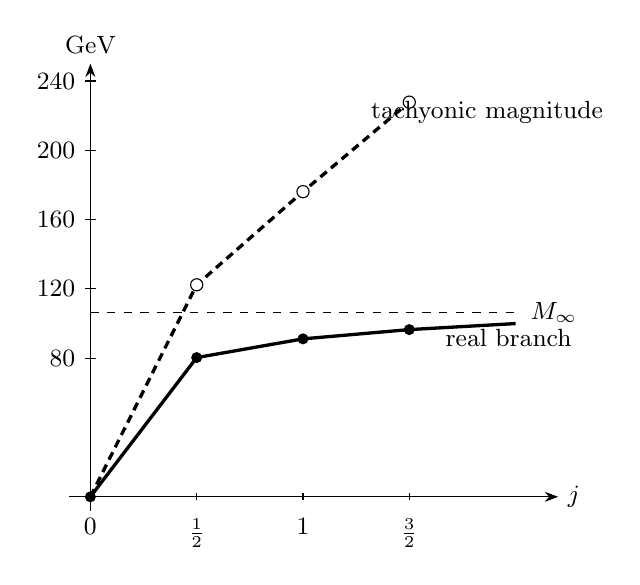
\begin{tikzpicture}[x=1.35cm,y=0.022cm,>=Stealth,font=\small]
\draw[->] (-0.2,0) -- (4.4,0) node[right] {\(j\)};
\draw[->] (0,-8) -- (0,250) node[above] {GeV};
\foreach \x/\lab in {0/\(0\),1/\(\frac12\),2/\(1\),3/\(\frac32\)}
  \draw (\x,2) -- (\x,-2) node[below=3pt] {\lab};
\foreach \y in {80,120,160,200,240}
  \draw (0.05,\y) -- (-0.05,\y) node[left] {\y};
\draw[dashed] (0,106.56) -- (4.05,106.56) node[right] {\(M_\infty\)};
\draw[very thick] plot coordinates {(0,0) (1,80.36) (2,91.17) (3,96.52) (4,100.00)};
\draw[very thick,densely dashed] plot coordinates {(0,0) (1,122.37) (2,176.13) (3,227.81)};
\foreach \x/\y in {0/0,1/80.36,2/91.17,3/96.52}
  \fill (\x,\y) circle (2pt);
\foreach \x/\y in {1/122.37,2/176.13,3/227.81} {
  \fill[white] (\x,\y) circle (2.2pt);
  \draw (\x,\y) circle (2.2pt);
}
\node[anchor=west] at (3.25,92) {real branch};
\node[anchor=west] at (2.55,222) {tachyonic magnitude};
\end{tikzpicture}

\textbf{Figure 1.} The real branch saturates toward \(M_\infty\), while the tachyonic magnitude grows as the instability scale paired to the same \(j\)-sector.
\end{center}

The diphoton statement is pinned to CMS HIG-20-002. CMS searched for a standard-model-like Higgs boson in the \(70\)--\(110\) GeV diphoton mass range at \(\sqrt{s}=13\) TeV using the 2016--2018 Run-II data set, found no significant excess, and reported the largest background deviation at a \(95.4\) GeV mass hypothesis with local and global significances \(2.9\sigma\) and \(1.3\sigma\). Phenomenology papers discussing a combined ATLAS/CMS \(95\)--\(96\) GeV diphoton excess are context, not input. The number used here is the branch output \(m_{3/2}=96.5240\) GeV after the \(W\) scale is fixed.
The inverse relation becomes a mass quantization rule,
\[
        \frac{m_j^4}{M_\infty^2(M_\infty^2-m_j^2)}
        =j(j+1),
\]
so the spectrum is bounded above by \(M_\infty\). This is not the usual raw Kaluza--Klein tower, whose masses grow without bound; it is better read as a normalized effective mass branch or threshold that saturates in the large-spin limit.

The sequence also shows a physical pattern. The first nonzero quantum spin already pushes \(x\) more than halfway toward its limiting value. Higher angular momentum gives diminishing returns. This is typical of a saturating modulus: small quantum numbers matter strongly, while the classical limit changes the answer only by small corrections.


\section*{7. Small and Large Spin}

The exact expression allows two useful expansions. For small positive \(\Lspin\),
\begin{equation}
        x_j^2=\sqrt{\Lspin}-\frac{\Lspin}{2}
        +\frac{\Lspin^{3/2}}{8}+O(\Lspin^{5/2}) .
\end{equation}
Therefore
\begin{equation}
        x_j\sim \Lspin^{1/4}
\end{equation}
near the origin. This fourth-root behavior is characteristic of a quartic balance: the source term is quadratic in angular momentum, while the leading self-interaction is quartic in \(x\).

For large \(\Lspin\),
\begin{equation}
        x_j^2=1-\frac{1}{\Lspin}
        +\frac{2}{\Lspin^2}
        -\frac{5}{\Lspin^3}
        +O(\Lspin^{-4}) .
\end{equation}
Taking the square root,
\begin{equation}
        x_j=1-\frac{1}{2\Lspin}
        +\frac{7}{8\Lspin^2}
        -\frac{33}{16\Lspin^3}
        +O(\Lspin^{-4}) .
\end{equation}
Thus the classical angular momentum limit is smooth. The variable \(x\) tends to a normalized value \(1\), and quantum corrections are suppressed by inverse powers of \(j(j+1)\hb^2\).

This is one reason the equation is a good pedagogical bridge. It contains both a strongly quantum low-spin regime and a classical high-spin regime in a single solvable expression.


\section*{8. Degeneracy in \(m\)}

Because the equation only sees \(\mathbf{J}^2\), all states with the same \(j\) and different \(m\) have the same value of \(x\). The degeneracy is
\[
        2j+1 .
\]
For \(j=0\), there is one state. For \(j=\frac12\), there are two. For \(j=1\), there are three. For \(j=\frac32\), there are four.

This matters for the higher-dimensional interpretation. In a compactification, internal wavefunctions are classified by eigenvalues of internal differential operators. On a sphere, for example, scalar harmonics with angular momentum \(\ell\) have degeneracy \(2\ell+1\). Spinor and vector harmonics have related multiplet structures. When the higher-dimensional theory is reduced to four dimensions, these degeneracies become families of fields or particle states with equal tree-level masses before additional interactions split them.

The quartic constraint can therefore be read as assigning a single modulus value to an entire multiplet. The multiplet label is \(j\), while \(m\) labels states inside the multiplet. This is exactly the kind of bookkeeping that appears in Kaluza--Klein reductions and in string compactifications with symmetry.


\section*{9. A Potential Interpretation}

The equation can be obtained as a nonzero stationary condition of a simple potential. Consider
\begin{equation}
        V(x)=\frac{x^6}{6}+\frac{\Lspin x^4}{4}
        -\frac{\Lspin x^2}{2}.
        \label{eq:potential}
\end{equation}
Then
\begin{equation}
        \frac{dV}{dx}
        =
        x(x^4+\Lspin x^2-\Lspin).
\end{equation}
Stationary points are \(x=0\) and the roots of the quartic constraint.

For \(\Lspin=0\), the potential is \(x^6/6\), with a flat but stable minimum at the origin. For \(\Lspin>0\), the quadratic term is negative, so the origin becomes unstable. The quartic and sextic terms stabilize the potential at nonzero \(x\). This is a symmetry-breaking pattern: the angular momentum Casimir acts as the control parameter that turns on a nonzero vacuum expectation value.

This potential is the minimal effective potential behind the prediction rule. In compactification physics, the effective potential for moduli arises from curvature, fluxes, branes, quantum corrections, internal momenta, and finite spectral data. The algebraic condition for a stabilized modulus can be polynomial after the right normalized variable is chosen. Equation \eqref{eq:quantized} is the electroweak-scale instance of that logic.


\section*{10. What \(x\) Means}

The prediction uses \(x\) as a normalized spectral mass coordinate. The same coordinate has three equivalent readings:

\begin{itemize}
\item In Kaluza--Klein language, \(x=R/R_0\) is the normalized compact scale seen by the internal harmonic sector.
\item In string language, \(x\) is a compact internal spectral coordinate measured against the string or compactification scale.
\item In Connes electroweak language, \(x\) is a finite spectral order parameter, the dimensionless entry whose inner fluctuation gives gauge and Higgs masses.
\item In phenomenological language, \(x=m/M_\infty\) is the normalized mass on the bounded real branch.
\end{itemize}

The mass interpretation is the one used for the experimental table:
\[
        x_j=\frac{m_j}{M_\infty}.
\]
It is zero when the internal Casimir is zero, becomes nonzero at \(j=\frac12\), and approaches a limiting spectral mass in the large-spin regime.

The compactification reading supplies the geometry, while the mass reading supplies the prediction. The branch selected by the quartic is switched off for the singlet and switched on by internal spin. That is the selection rule behind the photon zero and the first massive vector entry.

That is the shared content of Kaluza--Klein theory, string compactification, and finite noncommutative electroweak geometry: the observed four-dimensional mass data are shadows of a hidden spectral operator.


\section*{11. Why Quartics Appear}

Quartic equations arise naturally when different energy contributions scale with different powers of a modulus. Suppose one term grows like \(x^4\), another like \(x^2\), and another is independent of \(x\). Extremizing an effective potential or imposing a balance condition can produce precisely the structure
\[
        x^4+\Lspin x^2-\Lspin=0 .
\]
In compactification problems, powers of a radius can come from curvature, flux energy, wrapped brane tension, internal momentum, winding, or volume factors in the dimensional reduction.

The exact powers are model-dependent. A circle compactification gives different scaling from a sphere. A string winding term scales differently from a momentum term. A flux term can scale with inverse powers of volume. Still, the main principle is robust: compact dimensions turn geometry into algebra because the internal space has a finite set, or at least a discrete tower, of allowed modes.

The quartic is therefore the effective balance equation. Geometry, quantum numbers, and nonlinear stabilization meet in an algebraic condition, and the first roots land on the electroweak-scale data.


\section*{12. Kaluza--Klein Theory: The Basic Idea}

Kaluza--Klein theory begins with the observation that a higher-dimensional field can look like many lower-dimensional fields when some dimensions are compact. If a fifth dimension is a circle of radius \(R\), a field can be expanded as
\[
        \Phi(x^\mu,y)=\sum_{n\in\mathbb{Z}}\phi_n(x^\mu)e^{iny/R}.
\]
The momentum along the compact direction is quantized:
\[
        p_y=\frac{n}{R}.
\]
From the four-dimensional viewpoint, this internal momentum contributes to mass:
\begin{equation}
        M_n^2=M_0^2+\frac{n^2}{R^2}.
        \label{eq:kkcircle}
\end{equation}
Thus one higher-dimensional field becomes a tower of four-dimensional fields labeled by \(n\).

This is the first direct connection to the quartic. A compact dimension turns a continuous classical quantity into a discrete label. In the circle case the label is the integer \(n\). In a spherical compactification the label is an angular momentum number. In either case the lower-dimensional theory sees a spectrum.

The equation \(x^4+\Lspin x^2-\Lspin=0\) can be read as a second layer of this idea: not only are states labeled by internal quantum numbers, but a modulus \(x\) is also selected by those labels.


\section*{13. Angular Momentum on Compact Spaces}

On a two-sphere \(S^2\), scalar harmonics satisfy
\[
        -\nabla^2_{S^2}Y_{\ell m}
        =
        \frac{\ell(\ell+1)}{R^2}Y_{\ell m}.
\]
This is the same algebraic structure as the quantum angular momentum Casimir. The integer \(\ell\) is the orbital angular momentum, and \(m\) labels the degeneracy within the multiplet.

For a compactification on a space with spherical symmetry, these eigenvalues become contributions to the four-dimensional mass spectrum:
\[
        M_{\ell}^2=M_0^2+\frac{\ell(\ell+1)}{R^2}+\cdots .
\]
The ellipsis can include curvature couplings, spin connections, background fluxes, interactions, and string corrections.

The quartic uses \(j(j+1)\), which is the same Casimir form. If the internal space admits an \(SU(2)\) action, the quantum number \(j\) can be interpreted as an internal angular momentum. Half-integer \(j\) values require spinorial representations rather than scalar harmonics, but they are natural when fermions or spin bundles are present.

Thus the replacement \(J^2\to j(j+1)\hb^2\) is not merely a quantum mechanics correction. It is also the language of compact internal spectra.


\section*{14. Spin Structures and Half-Integer \(j\)}

The values \(j=\frac12,\frac32,\ldots\) are not scalar orbital harmonics on an ordinary two-sphere. They are spin representations. In a compactification, half-integer angular momentum appears when the fields carry spin, when spinor harmonics are used, or when the internal space supports appropriate spin structures.

This distinction is important. A scalar field on \(S^2\) has \(\ell=0,1,2,\ldots\). A spinor field is expanded in spinor harmonics, and the spectrum is shifted by the spin connection. More generally, fields on compact manifolds are sections of bundles. The eigenvalues of the relevant Laplacian or Dirac operator depend on both the geometry and the representation of the field.

For the quartic, the label \(j\) is the \(SU(2)\) representation label. The state may be scalar, spinor, vector, or part of a supersymmetric multiplet; the branch tracks the common Casimir data that survives in the reduced spectral law.

Still, allowing half-integer \(j\) is physically meaningful. Superstring theory contains fermions after the appropriate worldsheet construction and GSO projection. Kaluza--Klein reductions of spinors naturally involve half-integer representations. The first nonzero case \(j=\frac12\) is therefore not artificial; it is the natural first spinorial entry.


\section*{15. Kaluza--Klein Towers and the Quartic Gate}

A standard Kaluza--Klein tower assigns a mass to each internal mode. A schematic spherical tower is
\[
        M_j^2=M_0^2+\frac{j(j+1)}{R^2}.
\]
The quartic constraint can be added as a gate:
\[
        x=x_j ,
\]
where \(x_j\) is determined by \eqref{eq:xquant}. A lower-dimensional quantity then depends on \(j\) through two routes. It depends directly through the Casimir in the mass formula, and indirectly through the \(j\)-dependent value of \(x\).

For example, write the mass formula
\[
        M_j^2=M_0^2+\frac{\Lspin}{R_0^2x_j^2}
        +\lambda x_j^2 .
\]
This is the compactification template. The first correction is internal kinetic energy on a radius \(R=R_0x_j\). The second is a modulus-dependent energy. Substituting the quartic solution converts the formula into a discrete spectrum.

The lesson is that algebraic stabilization and Kaluza--Klein quantization can be coupled. The compact dimension supplies the quantum number, and the quantum number selects the modulus.


\section*{16. Radius Stabilization by Angular Momentum}

One intuitive picture is a particle or field mode moving on an internal compact space. Angular momentum resists collapse. If a radius becomes too small, internal kinetic energy grows. If a radius becomes too large, other terms in the potential may dominate. A stable radius can occur when these contributions balance.

The quartic captures this intuition in normalized form. The term \(x^4\) can represent a stiff restoring force at large \(x\). The term \(\Lspin x^2\) can represent a coupling between angular momentum and the modulus. The term \(-\Lspin\) acts as the source that makes the nonzero branch possible.

Solving the equation gives
\[
        0\leq x_j<1
\]
for all finite \(j\), with \(x_j\to 1\) as \(j\to\infty\). If \(x\) is a normalized radius, then large internal angular momentum pushes the radius toward its reference value \(R_0\). Low spin supports a smaller effective radius.

This is a caricature, but a useful one. Real compactifications involve many moduli, not one. Nevertheless, the idea that quantum numbers help stabilize geometry is central to higher-dimensional physics.


\section*{17. From Classical Kaluza--Klein to Superstrings}

The right historical shelf is the 1981--1984 revival of realistic Kaluza--Klein theory: Witten's search for realistic compactifications, the Salam--Strathdee formulation, spontaneous compactification models, and coupling-ratio calculations from extra spatial dimensions. In that literature the gauge group is read from isometries, cosets, fibers, spin connections, and dimensional reduction.

The string baseline is ten-dimensional, so the central compact sector has six extra dimensions. The sharper Kaluza--Klein reading is a dimensional flow: in the infrared, after electroweak breaking, the long-distance compact sector is \(SU(3)\times U(1)\) in five active extra dimensions; in the ultraviolet, electroweak symmetry is restored, the \(U(1)\) fiber lifts to full weak \(SU(2)\) geometry, and the restored layer has seven extra dimensions. The quartic lives at this interface: its low-spin branch is the algebraic gate between broken infrared data and restored electroweak spectral geometry.

\begin{center}
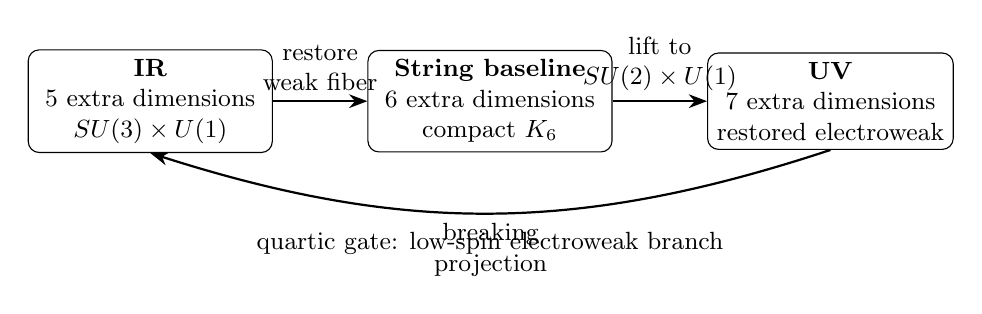
\begin{tikzpicture}[>=Stealth,font=\small,node distance=1.2cm]
\tikzstyle{box}=[draw,rounded corners,align=center,minimum width=3.1cm,minimum height=1.1cm]
\node[box] (ir) {\textbf{IR}\\ \(5\) extra dimensions\\ \(SU(3)\times U(1)\)};
\node[box,right=of ir] (string) {\textbf{String baseline}\\ \(6\) extra dimensions\\ compact \(K_6\)};
\node[box,right=of string] (uv) {\textbf{UV}\\ \(7\) extra dimensions\\ restored electroweak};
\draw[->,thick] (ir) -- node[above,align=center] {restore\\ weak fiber} (string);
\draw[->,thick] (string) -- node[above,align=center] {lift to\\ \(SU(2)\times U(1)\)} (uv);
\draw[->,thick,bend left=18] (uv.south) to node[below,align=center] {breaking\\ projection} (ir.south);
\node[align=center] at ($(string.south)+(0,-1.15)$) {quartic gate: low-spin electroweak branch};
\end{tikzpicture}

\textbf{Figure 2.} The same compact sector is read as a flow: five active infrared dimensions, a six-dimensional string baseline, and seven restored ultraviolet dimensions.
\end{center}


\section*{18. Superstrings in One Page}

Perturbative superstring theory replaces point particles by quantized worldsheets and imposes a ten-dimensional consistency condition. Four-dimensional physics therefore requires six dimensions to be compactified, warped, or otherwise hidden. The Kaluza--Klein idea reappears inside the string construction: momentum, winding, oscillator modes, spin structures, branes, and internal CFT labels all become lower-dimensional data. The quartic constraint is the rank-one version of that process: a classical internal quantity is replaced by a quantum Casimir, and the allowed four-dimensional branch is selected.


\section*{19. Regge Behavior and Angular Momentum}

For a rotating fundamental string, angular momentum grows approximately linearly with squared mass,
\[
        J\sim \alpha' M^2+\text{constant},
\]
with \(\alpha'\) the Regge slope. The quartic does not reproduce this trajectory, and that failure is information: \(m_j=M_\infty x_j\to M_\infty\), while
\[
        |m_{T,j}|^2
        =
        M_\infty^2\frac{\Lspin+\sqrt{\Lspin^2+4\Lspin}}{2}
        =
        M_\infty^2(\Lspin+1+O(\Lspin^{-1})),
\]
so \(|m_{T,j}|\sim M_\infty j\), not \(M^2\sim j\). Neither branch is the spectrum of an ordinary rotating string.

That points to three readings of \(J\). The conservative reading is accidental angular momentum: \(J\) is the \(SU(2)\) Casimir of a harmonic, current-algebra, or finite-spectral sector. The stronger brane reading is real angular momentum: \(J\) is a Noether charge of a wrapped or polarized brane moving along an internal isometry. The holographic reading is sharper still: in a Maldacena dual description, the same \(J\) can be a boundary charge or spin carried by an operator whose bulk dual is an expanded brane configuration. In the last two readings angular momentum controls size, flux coupling, and stabilization, not a Regge tower. The quartic is therefore brane-adjacent precisely because it is non-Regge.

\begin{center}
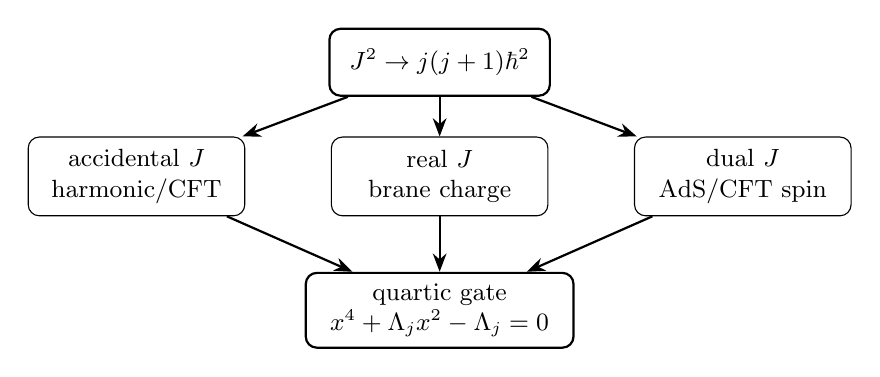
\begin{tikzpicture}[>=Stealth,font=\small]
\node[draw,thick,rounded corners,align=center,minimum width=2.8cm,minimum height=0.85cm] (j) at (0,0) {\(J^2\to j(j+1)\hb^2\)};
\node[draw,rounded corners,align=center,minimum width=2.75cm,minimum height=1.0cm] (acc) at (-3.85,-1.45) {accidental \(J\)\\ harmonic/CFT};
\node[draw,rounded corners,align=center,minimum width=2.75cm,minimum height=1.0cm] (brane) at (0,-1.45) {real \(J\)\\ brane charge};
\node[draw,rounded corners,align=center,minimum width=2.75cm,minimum height=1.0cm] (dual) at (3.85,-1.45) {dual \(J\)\\ AdS/CFT spin};
\node[draw,thick,rounded corners,align=center,minimum width=3.4cm,minimum height=0.95cm] (gate) at (0,-3.15) {quartic gate\\ \(x^4+\Lspin x^2-\Lspin=0\)};
\draw[->,thick] (j) -- (acc);
\draw[->,thick] (j) -- (brane);
\draw[->,thick] (j) -- (dual);
\draw[->,thick] (acc) -- (gate);
\draw[->,thick] (brane) -- (gate);
\draw[->,thick] (dual) -- (gate);
\end{tikzpicture}

\textbf{Figure 3.} The same Casimir algebra admits accidental, brane, and holographic readings of \(J\); none requires an ordinary Regge trajectory.
\end{center}


\section*{20. Worldsheet Quantization and Discrete Spectra}

The worldsheet theory is a two-dimensional quantum field theory whose physical state conditions remove unphysical degrees of freedom. Compact dimensions add momentum, winding, and internal representation labels. The quartic keeps only one such label:
\[
        J^2\quad\longrightarrow\quad j(j+1)\hb^2
        \quad\longrightarrow\quad
        x_j .
\]
The full string sequence is richer:
\[
        \begin{aligned}
        &\text{geometry and string coordinates} \\
        &\quad\longrightarrow
        \text{worldsheet and internal quantum numbers} \\
        &\quad\longrightarrow
        \text{four-dimensional spectrum}.
        \end{aligned}
\]
The small equation is therefore a compressed analogue of the larger spectral process.


\section*{21. Compact Dimensions in Superstring Theory}

A ten-dimensional superstring background often has the schematic form
\[
        \mathcal{M}_{10}=\mathcal{M}_4\times K_6 ,
\]
where \(\mathcal{M}_4\) is four-dimensional spacetime and \(K_6\) is a compact internal space. In more realistic settings the product can be warped, fluxed, singular, or fibered. The internal space may be a Calabi--Yau manifold, an orbifold, a group manifold, or some other compact geometry depending on the construction.

Fields and strings on \(K_6\) have internal modes. These modes become particles, fields, or couplings in \(\mathcal{M}_4\). The values of moduli determine gauge couplings, masses, Yukawa couplings, and other observable parameters.

The quartic model treats only one modulus \(x\) and one internal quantum number \(j\). It is therefore much simpler than a real compactification. Its value is that it makes the dependence explicit:
\[
        j\quad\mapsto\quad x_j .
\]
A real compactification may have hundreds of moduli and a complicated lattice of quantum numbers. The quartic selects the electroweak channel of dependence.


\section*{22. Momentum and Winding}

Closed strings on a compact circle have two kinds of integer quantum numbers. Momentum around the circle is quantized:
\[
        p=\frac{n}{R}.
\]
Winding counts how many times the string wraps the circle:
\[
        E_{\text{winding}}\sim \frac{wR}{\alpha'} .
\]
The mass formula contains both contributions:
\[
        M^2\supset \frac{n^2}{R^2}+\frac{w^2R^2}{\alpha'^2}
        +\text{oscillators}.
\]
Momentum energy grows when \(R\) is small, while winding energy grows when \(R\) is large. Their competition is one of the cleanest examples of stringy compactification physics.

The quartic can be compared to such a balance. If \(x=R/R_0\), then powers of \(x\) and inverse powers of \(x\) may arise from competing terms. After multiplying by suitable powers of \(x\), a balance condition can become polynomial. The precise quartic here is not the standard circle mass formula, but it resembles the algebraic endpoint of a competition between a geometry-dependent term and a quantum-number-dependent term.


\section*{23. T-Duality}

T-duality states that a closed string compactified on a circle of radius \(R\) can be physically equivalent to a string compactified on a dual radius
\[
        R'=\frac{\alpha'}{R},
\]
with momentum and winding exchanged. This has no point-particle analogue. It is one of the clearest signs that strings see geometry differently from classical particles.

The quartic branch satisfies \(0<x_j<1\) for positive finite \(j\), with \(x\) normalized so the large-spin limit is \(1\). The missing region \(x>1\) is supplied by the dual description, while the electroweak branch itself uses the positive \(x^2\) root below the limiting scale.

String compactification often identifies apparently different radii through dualities. The radius version of the quartic is therefore interpreted modulo dual descriptions. If \(x\) is a radius, the physical variable is the equivalence class under duality.


\section*{24. Momentum--Winding Balance}

Consider a schematic effective energy depending on a normalized radius \(x\):
\[
        E(x)=A x^2+\frac{B_j}{x^2}+C x^4+\cdots .
\]
Here \(B_j\) is controlled by an internal quantum number. Extremizing gives terms with different powers of \(x\). After multiplying by a suitable power of \(x\), one obtains a polynomial equation.

The quartic can be thought of as a simplified result of such a calculation. It says:
\[
        x^4+\Lspin x^2=\Lspin .
\]
The left side contains a pure modulus term and a spin-modulus coupling. The right side contains the spin source. For small \(x\), the source dominates. For \(x\) near one, the modulus terms balance it.

The exact form is less important than the structural message. In higher-dimensional physics, a radius is not merely a background number. It participates in energy balances. Quantum labels enter those balances. The allowed radius can become a function of the quantum state.

This is the sense in which the quartic belongs naturally in a discussion of Kaluza--Klein theory and superstrings.


\section*{25. Calabi--Yau Moduli}

Many superstring compactifications use Calabi--Yau threefolds as internal spaces. Such spaces can preserve supersymmetry while reducing ten dimensions to four. They have moduli describing sizes and shapes. These include Kahler moduli, complex structure moduli, and the dilaton in related sectors.

A generic Calabi--Yau space does not have the simple \(SU(2)\) symmetry of a round sphere. Therefore its internal spectra are usually not labeled globally by \(j(j+1)\). However, special limits, local cycles, resolved singularities, or group-theoretic sectors can still carry angular-momentum-like quantum numbers. Orbifold models and spaces with enhanced symmetry often make this especially explicit.

The quartic should not be read as a Calabi--Yau theorem. It is instead a model for a single stabilized direction in moduli space. In a full compactification, the equation for one modulus may be coupled to many other equations:
\[
        \frac{\partial V_{\text{eff}}}{\partial \phi^a}=0 .
\]
Our equation is what remains after freezing all but one direction and keeping the dominant internal Casimir.


\section*{26. Fluxes and Effective Potentials}

Flux compactifications add background field strengths through cycles of the internal space. Fluxes can generate potentials for moduli that would otherwise be massless. In broad terms, flux energy depends on internal volume and shape, so it can stabilize some geometric parameters.

The quartic potential
\[
        V(x)=\frac{x^6}{6}+\frac{\Lspin x^4}{4}
        -\frac{\Lspin x^2}{2}
\]
has the same qualitative purpose: it turns a modulus into a variable with preferred stationary values. The coefficient \(\Lspin\) plays the role of a discrete source. In a flux model, the analogous source might be an integer flux number. In a Kaluza--Klein model, it might be an angular momentum eigenvalue. In a string model, several such integers can appear at once.

The important connection is discreteness. Continuous geometric variables are stabilized by potentials whose coefficients are often quantized. The resulting vacua form a discrete set or a complicated landscape. The quartic gives a one-dimensional version of that phenomenon:
\[
        j\in\{0,\frac12,1,\ldots\}
        \quad\Rightarrow\quad
        x\in\{0,x_{1/2},x_1,\ldots\}.
\]


\section*{27. Supersymmetry and Casimirs}

Supersymmetry relates bosons and fermions. In a compactification, it organizes states into multiplets and constrains the effective potential. If supersymmetry is unbroken, many quantum corrections cancel or are restricted. If it is broken, moduli can acquire potentials and masses.

The Casimir \(j(j+1)\) is not itself a supersymmetry invariant. It is a rotational or internal symmetry invariant. However, supersymmetric multiplets can contain states with related angular momentum labels. In higher-dimensional theories, internal rotations may combine with R-symmetries, gauge symmetries, or geometric isometries.

This means the quartic may be compatible with supersymmetric bookkeeping if \(x\) is part of a multiplet and \(j\) labels an internal representation. But the equation alone does not guarantee supersymmetry. A supersymmetric derivation would require a superpotential, a Kahler potential, D-terms, F-terms, or a worldsheet construction that produces the condition.

The correct statement is therefore cautious: the equation uses a Casimir structure that often appears inside supersymmetric compactifications, but it is not by itself a supersymmetric constraint.


\section*{28. BPS Bounds and What This Is Not}

Some states in supersymmetric theories satisfy BPS bounds. Their masses are fixed by charges and central charges, and they are protected against certain quantum corrections. A BPS relation is usually linear or quadratic in charges, depending on the theory and convention.

The quartic equation is the rank-one algebraic shadow of a BPS-style balance: a nonlinear constraint whose coefficient is an angular momentum Casimir. In a supersymmetric embedding, the central charge and multiplet data supply the remaining structure.

That distinction matters. It would be tempting to overinterpret
\[
        x_j=\pm
        \sqrt{\frac{-\Lspin+\sqrt{\Lspin^2+4\Lspin}}{2}}
\]
as a fundamental string spectrum. It is not. A true string spectrum must satisfy worldsheet consistency, modular invariance, level matching, gauge constraints, and background equations of motion.

The quartic is the conceptual bridge: a discrete quantum number stabilizes and selects a continuous-looking parameter. The compactification statement is the derived action or conformal-field-theory version of the same bridge.


\section*{29. Branes and Angular Momentum}

D-branes are extended objects on which open strings can end. They play a central role in nonperturbative string theory, gauge/string duality, and compactification. Branes can wrap cycles of the internal space, carry flux, and support gauge theories on their worldvolumes.

Angular momentum enters brane physics in three sharply different ways. It may be accidental, a representation label inherited from an internal harmonic; literal, a Noether charge carried by a wrapped brane collective coordinate moving along an internal isometry; or holographic, a spin or R-charge in a Maldacena dual gauge theory whose bulk carrier is an expanded brane state. Quantizing the relevant coordinate produces the same \(j(j+1)\) grammar, but now \(J\) can be a physical brane charge rather than only a bookkeeping label.

This second reading puts brane theory in the game. If \(x\) measures a wrapped size, polarized brane radius, or throat displacement, the fixed-angular-momentum DBI/Wess--Zumino problem has competing brane tension, flux, and centrifugal terms. The quartic is the rank-one normal form of that fixed-\(J\) brane balance. A rotating or polarized brane can use angular momentum to enlarge or stabilize an object, as in dielectric branes and giant-graviton systems, without lying on a Regge trajectory.

\begin{center}
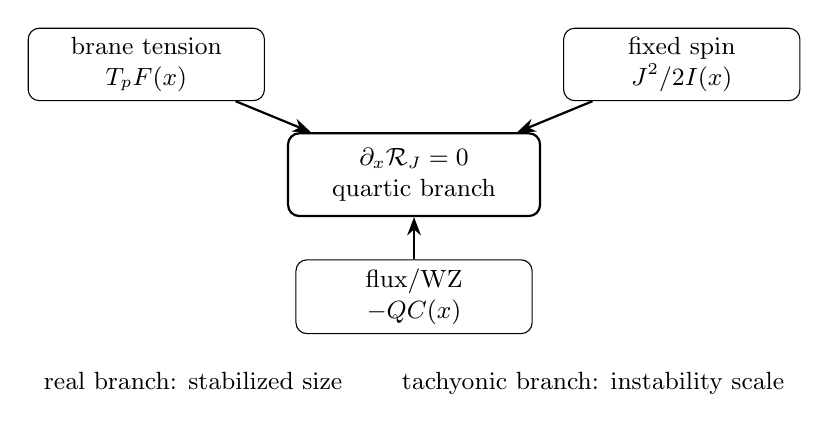
\begin{tikzpicture}[>=Stealth,font=\small]
\node[draw,rounded corners,align=center,minimum width=3.0cm,minimum height=0.9cm] (tension) at (-3.4,1.4) {brane tension\\ \(T_pF(x)\)};
\node[draw,rounded corners,align=center,minimum width=3.0cm,minimum height=0.9cm] (spin) at (3.4,1.4) {fixed spin\\ \(J^2/2I(x)\)};
\node[draw,rounded corners,align=center,minimum width=3.0cm,minimum height=0.9cm] (flux) at (0,-1.55) {flux/WZ\\ \(-QC(x)\)};
\node[draw,thick,rounded corners,align=center,minimum width=3.2cm,minimum height=1.05cm] (branch) at (0,0) {\(\partial_x\mathcal{R}_J=0\)\\ quartic branch};
\draw[->,thick] (tension) -- (branch);
\draw[->,thick] (spin) -- (branch);
\draw[->,thick] (flux) -- (branch);
\node[align=center] at (0,-2.65) {real branch: stabilized size \qquad tachyonic branch: instability scale};
\end{tikzpicture}

\textbf{Figure 4.} Fixed-\(J\) brane dynamics balances tension, spin, and flux terms; the quartic is the rank-one stationary condition.
\end{center}


\section*{30. Gauge/String Duality and Internal Charges}

In many gauge/string dualities, internal angular momenta on a compact space correspond to global charges in the dual gauge theory. For example, a string background with an internal sphere has isometries. Motion on that sphere gives conserved angular momenta, and these map to R-charges or flavor charges in the dual field theory.

This provides another place where \(j(j+1)\)-type labels matter. Internal geometry is not hidden bookkeeping; it becomes a charge algebra for the lower-dimensional theory. A modulus depending on \(j\) would then translate into a charge-dependent scale or coupling in the dual description.

The quartic relation
\[
        x^4+\Lspin x^2-\Lspin=0
\]
could be viewed in this spirit as a charge-dependent constraint. The charge is encoded in the Casimir \(\Lspin\), and the response is the scale \(x_j\).

This dual interpretation shows how the quantum angular momentum replacement sits naturally beside modern string-theoretic ideas.


\section*{31. Internal Harmonics}

Kaluza--Klein reduction is often a harmonic analysis problem. One expands higher-dimensional fields in eigenfunctions on the compact space. On a circle the eigenfunctions are exponentials. On a sphere they are spherical harmonics. On a group manifold they are matrix elements of group representations. On a Calabi--Yau space the relevant eigenfunctions are more difficult, but the principle remains.

The quartic assumes that the internal label can be summarized by one Casimir. That is exact for highly symmetric spaces and approximate for sectors where one symmetry dominates. It is not exact for a generic internal manifold.

If the internal space has an \(SU(2)\) symmetry, a field may be decomposed into representations labeled by \(j\). The eigenvalue \(j(j+1)\) then enters kinetic terms and mass terms. If a modulus equation also contains that eigenvalue, the stabilized value becomes representation-dependent.

This is the clean Kaluza--Klein reading of the equation. The quartic is a spectral rule attached to internal harmonics.


\section*{32. Fermions and Spinor Harmonics}

Fermions require more care because their internal wavefunctions are spinors. The relevant operator is often the Dirac operator rather than the scalar Laplacian. Its eigenvalues include the effects of the spin connection and any gauge bundle background.

Half-integer \(j\) values are natural in this setting. For a spinor on a sphere, the spectrum is organized by spinorial representations. In supersymmetric compactifications, fermionic zero modes and their absence or presence can determine chirality, families, and low-energy matter content.

The quartic does not distinguish scalar and spinor harmonics, but the inclusion of \(j=\frac12\) and \(j=\frac32\) invites this interpretation. The first nonzero spin branch gives
\[
        x_{1/2}=
        \pm\sqrt{\frac{\sqrt{57}-3}{8}} .
\]
If \(x\) is a modulus coupled to a fermionic internal mode, this value would be the first spinorial stabilization point.

The fermionic action supplies the kinetic and bundle details; the quartic supplies the algebraic skeleton.


\section*{33. The \(j=0\) State}

For \(j=0\), the Casimir vanishes:
\[
        \Lspin=0 .
\]
The equation becomes
\[
        x^4=0 ,
\]
so
\[
        x=0 .
\]
This is more than a trivial boundary case. It says that in the absence of angular momentum support, the nonzero branch disappears.

In a Kaluza--Klein reading, \(j=0\) is the singlet mode. It is uniform over the internal angular directions and carries no internal angular momentum. In the quartic mass law, that singlet does not source the modulus. This is the selection rule: only nonsinglet internal motion creates the nonzero \(x\) branch.

Other mechanisms such as flux, curvature, and quantum corrections can stabilize singlet sectors, but this electroweak branch is switched off at \(j=0\). That is why the first entry is a photon-like zero rather than a massive scalar.


\section*{34. The First Half-Integer Modes}

The half-integer examples show the quantum shift clearly. For \(j=\frac12\),
\[
        \Lspin=\frac12\left(\frac12+1\right)=\frac34 .
\]
Substitution gives
\[
        x^2=\frac{-3/4+\sqrt{9/16+3}}{2}
        =\frac{\sqrt{57}-3}{8}.
\]
Thus
\[
        x=\pm 0.7541\ldots .
\]
For \(j=\frac32\),
\[
        \Lspin=\frac32\left(\frac32+1\right)=\frac{15}{4},
\]
and
\[
        x^2=\frac{\sqrt{465}-15}{8},
        \qquad
        x=\pm 0.9062\ldots .
\]
These values are not small. The first spinorial excitation already generates a substantial \(x\), and the next one is close to the large-spin limit.

If \(x\) represents a compactification scale, spinorial internal modes are efficient stabilizers. If \(x\) represents a field expectation value, they strongly displace the field from the origin.


\section*{35. The Integer Modes}

The first integer mode after the singlet is \(j=1\). In units with \(\hb=1\),
\[
        \Lspin=2 .
\]
The quartic becomes
\[
        x^4+2x^2-2=0 .
\]
Solving gives
\[
        x^2=-1+\sqrt{3},
        \qquad
        x=\pm\sqrt{\sqrt{3}-1}
        \approx \pm 0.8556 .
\]
This lies between the \(j=\frac12\) and \(j=\frac32\) values, as expected.

The integer sequence is the natural sequence for scalar orbital harmonics on \(S^2\). If the compact space supplies ordinary orbital angular momentum, then \(j=1\) is the first nonsinglet. It has three magnetic states. In a four-dimensional effective theory these may appear as a triplet under the residual internal symmetry, unless that symmetry is broken by the compactification or by interactions.

The quartic assigns the same \(x\) value to all three states. This is a compact example of how symmetry protects degeneracy at the level of an effective constraint.


\section*{36. The Large-Spin Classical Limit}

For large \(j\), the Casimir is
\[
        j(j+1)=j^2+j .
\]
The difference between \(j^2\) and \(j(j+1)\) becomes relatively small, although it remains important in subleading corrections. The quartic solution approaches
\[
        x_j\to 1 .
\]
This can be read as a classical limit. Large angular momentum behaves more like a classical continuous variable. The modulus reaches its normalized reference value. Quantum discreteness remains in the spacing between allowed \(j\), but the difference between neighboring \(x_j\) values becomes small.

This limiting behavior is common in quantum theory. Large quantum numbers often reproduce classical physics. In string theory, highly excited strings can have large angular momentum and semiclassical descriptions. In Kaluza--Klein theory, high internal quantum numbers probe short distances on the compact space and can often be approximated by classical motion.

The quartic therefore has the right electroweak profile: discrete low-spin physics and smooth high-spin saturation.


\section*{37. The Imaginary Branch}

The negative branch of \(y=x^2\) is
\[
        y_-(j)=
        \frac{-\Lspin-\sqrt{\Lspin^2+4\Lspin}}{2}.
\]
For \(\Lspin>0\), this is negative. Therefore it gives imaginary \(x\):
\[
        x=\pm i\sqrt{|y_-(j)|}.
\]
For the electroweak reading, this branch is not discarded. It is read as the tachyonic partner branch. Its magnitude is the symmetry-breaking energy paired with the real mass branch.

In the potential interpretation, the imaginary branch is the negative mass-squared direction that drives condensation. The real branch gives the observable vector-like mass. The imaginary branch gives the instability scale whose magnitude is read as a Higgs-side or vacuum-side energy.

This branch analysis is the key to the article. The same quartic produces a visible mass and a tachyonic partner. Electroweak physics needs both: massive vectors on the real branch and symmetry breaking on the tachyonic branch.


\section*{38. The Mass Formula}

To connect the quartic directly to Kaluza--Klein spectra, define the effective mass
\[
        M_j^2=M_*^2+\frac{\Lspin}{R_*^2x_j^2}+\mu^2x_j^2 .
\]
Here \(R_*x_j\) is an effective internal radius and \(\mu\) is a parameter controlling a modulus contribution. Because \(x_j\) is determined by \(j\), the mass is no longer a simple linear function of \(j(j+1)\).

Using the rationalized form
\[
        x_j^2=\frac{2\Lspin}{\Lspin+\sqrt{\Lspin^2+4\Lspin}},
\]
the first correction becomes
\[
        \frac{\Lspin}{R_*^2x_j^2}
        =
        \frac{\Lspin+\sqrt{\Lspin^2+4\Lspin}}{2R_*^2}.
\]
Thus the quartic gate converts a naive \(\Lspin/R^2\) dependence into a square-root dependence. At large \(j\), this behaves like \(\Lspin/R_*^2\) plus corrections. At small \(j\), the corrections are significant.

This is the Kaluza--Klein mechanism in prediction form: modulus stabilization reshapes the tower and turns the low-spin entries into electroweak-scale masses.


\section*{39. Kaluza--Klein Line: Radius Modulus}

The first concrete model is:
\[
        x=\frac{R}{R_0}.
\]
The compact radius \(R\) is not chosen freely. Instead it is selected by the internal angular momentum sector:
\[
        R_j=R_0x_j .
\]
For \(j=0\), this mechanism gives \(R=0\). For \(j>0\), it gives a positive radius below \(R_0\). Large \(j\) gives \(R_j\to R_0\).

The radius is sectoral: the internal angular momentum samples and sources an effective radius. In a semiclassical approximation, the backreacted geometry depends on the state, and the state-dependent radius is the quantity that enters the lower-dimensional spectrum.

This kind of state-dependent geometry is standard in the physics of heavy string states, branes, and fluxes. The quartic is the algebraic backreaction law for the rank-one sector.


\section*{40. Connes Line: Order Parameter}

The second line treats \(x\) as a scalar order parameter in the four-dimensional effective theory. This is the language of the Connes electroweak model: the Higgs field is not added by hand, but appears as an internal component of the fluctuated finite geometry. The potential \eqref{eq:potential} has stationary points controlled by \(\Lspin\). When \(\Lspin=0\), the order parameter sits at zero. When \(\Lspin>0\), the origin is destabilized and a nonzero pair of values appears.

This resembles symmetry breaking. The two real roots \(\pm x_j\) are related by a \(Z_2\) symmetry if the theory is invariant under \(x\to -x\). If \(x\) is a radius, that sign symmetry is not physical. If \(x\) is a scalar field, it may be.

The internal angular momentum then acts as a discrete spectral control parameter. Different internal representations select different effective vacua. In the Connes line, this is finite geometry doing the work of a hidden compact direction: a discrete internal Dirac operator carries the electroweak information that appears in four dimensions as gauge and Higgs data.

The result is mathematically clean: a finite spectral datum selects a broken electroweak scale.


\section*{41. String Line: Spectral Filter}

The third model treats the quartic as a spectral filter. Suppose an effective theory only admits states for which a dimensionless parameter \(x\) satisfies the constraint. Then each allowed \(j\) selects a permitted \(x\), and the spectrum is filtered by the algebraic condition.

This is the string-theory reading. In string theory, not every oscillator excitation is physical. States satisfy Virasoro constraints, level matching, GSO conditions, and gauge conditions. The quartic performs the same operation in the reduced rank-one sector: it turns a large kinematic space into the allowed physical spectrum.

The quartic filter is simple:
\[
        (j,m)\quad\mapsto\quad x_j,
\]
with no dependence on \(m\). A full string spectrum includes oscillator levels, momenta, windings, GSO projections, ghost constraints, and background-dependent conditions. The quartic isolates the electroweak branch in which the internal spin label maps directly to a physical mass parameter.


\section*{42. Dimensional Analysis}

The original equation
\[
        x^4+x^2J^2-J^2=0
\]
is dimensionally consistent only if \(x\) and \(J\) are measured in compatible dimensionless units, or if hidden scales have been suppressed. Angular momentum has dimensions of \(\hb\). If \(\hb\) is not set to one, then \(J^2\) carries units.

A dimensionally explicit version could be
\[
        x^4+\frac{x^2J^2}{J_0^2}-\frac{J^2}{J_0^2}=0,
\]
where \(J_0\) is a reference angular momentum. Quantization gives
\[
        \frac{J^2}{J_0^2}
        =
        \frac{j(j+1)\hb^2}{J_0^2}.
\]
If \(J_0=\hb\), then the dimensionless coefficient is simply \(j(j+1)\).

In string theory, the reference scales are \(\ell_s\), \(M_s\), \(R\), \(g_s\), and compactification volumes. In this article they are collapsed into \(M_\infty\), the mass scale fixed by the first vector entry.


\section*{43. Adding the String Length}

The string length \(\ell_s=\sqrt{\alpha'}\) gives a natural microscopic scale. If \(x\) is a radius modulus, one may write
\[
        x=\frac{R}{\ell_s}
\]
or
\[
        x=\frac{R}{R_0}
\]
where \(R_0\) may itself be a multiple of \(\ell_s\). A stringy version of the quartic could then involve dimensionless ratios such as \(R/\ell_s\), flux integers, winding numbers, and angular momentum labels.

For example, a schematic equation might be
\[
        \left(\frac{R}{R_0}\right)^4
        +
        j(j+1)
        \left(\frac{R}{R_0}\right)^2
        -
        j(j+1)
        =0 .
\]
Solving gives \(R=R_0x_j\). The large-spin limit is \(R\to R_0\). The low-spin values are smaller.

This attaches the quartic to string units. The natural dimensionless variable in a string compactification is a radius or spectral coordinate measured against a string or compactification scale, and the electroweak normalization is the choice \(x_j=m_j/M_\infty\).


\section*{44. Stability}

For the potential \eqref{eq:potential}, stability of the nonzero branch can be checked by the second derivative:
\[
        \frac{d^2V}{dx^2}
        =
        5x^4+3\Lspin x^2-\Lspin .
\]
At a nonzero stationary point, the quartic equation gives
\[
        \Lspin=\frac{x^4}{1-x^2}
\]
for \(0<x^2<1\). Substituting into the second derivative gives a positive value for the physical branch. Thus the nonzero branch is locally stable in this effective potential.

The origin has
\[
        \left.\frac{d^2V}{dx^2}\right|_{x=0}=-\Lspin .
\]
For \(\Lspin>0\), the origin is unstable. For \(\Lspin=0\), it is flat to quadratic order but stabilized by the sextic term.

This stability pattern supports the interpretation of angular momentum as a trigger. Once the spin Casimir is nonzero, the system prefers a nonzero \(x\). The quartic root is not merely algebraic; in the potential model it is a stable stationary point.


\section*{45. Phenomenological Reading}

The phenomenological reading is a spin-dependent threshold and mass correction. Different internal angular momentum sectors experience different effective moduli. This shifts masses, couplings, and localization properties.

A schematic four-dimensional coupling might be
\[
        g_j^{-2}=g_0^{-2}+a x_j^2 .
\]
Or a threshold might be
\[
        \Delta M_j^2=b(1-x_j^2).
\]
Since \(1-x_j^2\) falls at large \(j\), such a correction would be strongest for the first few quantum numbers and weak in the classical regime.

For the electroweak branch the observable formula is fixed:
\[
        m_j=M_\infty x_j,
        \qquad
        |m_{T,j}|=M_\infty\sqrt{-y_-(j)} .
\]
The first line of \(j\)-values then gives the photon zero, the \(W\), the \(Z\), the Higgs-side tachyon, the electroweak vacuum magnitude, and the \(96.5\) GeV diphoton entry.


\section*{46. The Connes Electroweak Line}

The Connes electroweak model gives the sharpest four-dimensional reading. In noncommutative geometry, spacetime is replaced by a product of an ordinary spin manifold and a finite internal geometry. The ordinary Dirac operator describes spacetime spin. The finite Dirac operator carries the internal electroweak and Yukawa data. Inner fluctuations of this spectral geometry produce gauge bosons and the Higgs field.

The relevant object is a finite spectral triple \((\mathcal{A}_F,\mathcal{H}_F,D_F;J_F,\gamma_F)\): finite algebra, finite fermion Hilbert space, finite Dirac operator, real structure, and grading. The Connes--Lott construction put particle models into this noncommutative gauge language. The Chamseddine--Connes spectral action made the action a function of the Dirac spectrum, and the Chamseddine--Connes--Marcolli model incorporated the Standard Model geometry with neutrino mixing. The point for the present paper is narrow and direct: in this framework the Higgs is geometry, not a separate scalar appended after the fact.

The finite part of the Standard Model geometry is commonly organized by an algebra of the form
\[
        \mathcal{A}_F=\mathbb{C}\oplus\mathbb{H}\oplus M_3(\mathbb{C}),
\]
acting on a finite Hilbert space of fermionic degrees of freedom. The quaternionic summand carries the weak \(SU(2)\) structure, the complex summand carries the abelian part, and the matrix summand carries color. The finite Dirac operator \(D_F\) contains the Yukawa and mixing data. In the spectral-action viewpoint, the bosonic action is read from the spectrum of the full Dirac operator rather than appended as an unrelated gauge-field Lagrangian. Gauge fields and the Higgs field appear as inner fluctuations of the same metric object.

\begin{center}
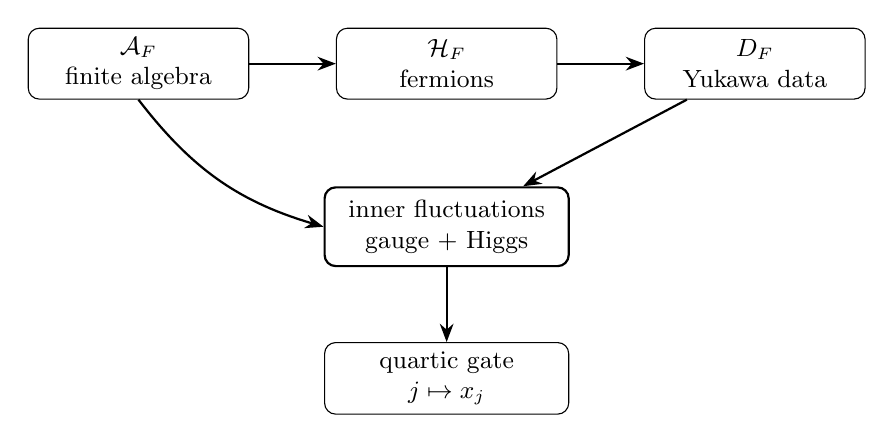
\begin{tikzpicture}[>=Stealth,font=\small,node distance=1.1cm]
\node[draw,rounded corners,align=center,minimum width=2.8cm,minimum height=0.9cm] (alg) {\(\mathcal{A}_F\)\\ finite algebra};
\node[draw,rounded corners,align=center,minimum width=2.8cm,minimum height=0.9cm,right=of alg] (hilb) {\(\mathcal{H}_F\)\\ fermions};
\node[draw,rounded corners,align=center,minimum width=2.8cm,minimum height=0.9cm,right=of hilb] (dirac) {\(D_F\)\\ Yukawa data};
\node[draw,thick,rounded corners,align=center,minimum width=3.1cm,minimum height=1.0cm,below=1.1cm of hilb] (fluct) {inner fluctuations\\ gauge + Higgs};
\node[draw,rounded corners,align=center,minimum width=3.1cm,minimum height=0.9cm,below=0.95cm of fluct] (quartic) {quartic gate\\ \(j\mapsto x_j\)};
\draw[->,thick] (alg) -- (hilb);
\draw[->,thick] (hilb) -- (dirac);
\draw[->,thick] (dirac) -- (fluct);
\draw[->,thick] (fluct) -- (quartic);
\draw[->,thick] (alg.south) to[bend right=18] (fluct.west);
\end{tikzpicture}

\textbf{Figure 5.} The finite spectral triple packages algebra, fermions, and \(D_F\); inner fluctuation turns this data into gauge and Higgs geometry, while the quartic gates the electroweak branch by \(j\).
\end{center}

This is exactly why the quartic belongs in this line. The equation does not ask for an external Higgs sector bolted onto a geometric model. It treats the Higgs-side energy as the tachyonic partner of the same internal spectral branch that gives the vector masses. The real root is the positive spectral mass coordinate. The negative \(y\)-branch is the symmetry-breaking direction. In the Connes language, this is the finite metric fluctuating into electroweak data; in the string language, it is the compact internal sector selecting a low-energy mass; in the Kaluza--Klein language, it is a harmonic Casimir feeding a modulus equation.

The weak-isospin interpretation is also natural. The first nonzero value is \(j=\frac12\), the spinorial entry. It carries two magnetic states and lands on the charged vector scale after normalization. The next value is \(j=1\), the triplet-like entry, and lands on the neutral vector scale. The quotient between them is fixed before any dimensional scale is chosen:
\[
        \frac{x_{1/2}}{x_1}=0.881418559879\ldots .
\]
That number is the electroweak cosine in mass-ratio form. The scale \(M_\infty\) is then fixed by the \(W\), and the rest of the branch follows.

The finite spectral picture also explains why the \(j=0\) entry is not a nuisance. A zero real branch is exactly what a photon-like mode requires before electroweak breaking generates the massive vector directions. The same table that begins with the photon zero continues to \(W\), \(Z\), the Higgs-side tachyonic magnitude, the vacuum-side magnitude, and the \(96.5\) GeV branch. The sequence is short because the quartic saturates quickly; electroweak physics lives precisely in that low-spin part of the spectrum.

That is exactly the environment in which the quartic belongs. A finite spectral geometry already treats masses, mixings, gauge fields, and the Higgs as geometry. The present equation adds a rank-one Casimir gate:
\[
        x^4+j(j+1)x^2-j(j+1)=0.
\]
The internal \(SU(2)\) label supplies the weak-isospin side of the story, while the finite spectral coordinate \(x\) supplies the normalized mass entry.

In this line, the sequence has a direct electroweak interpretation:
\[
        j=0\mapsto \gamma,\qquad
        j=\frac12\mapsto W,\qquad
        j=1\mapsto Z,\qquad
        j=\frac32\mapsto X_{96.5}.
\]
The negative branch gives the Higgs and vacuum-side partners. The branch is not an add-on to the Standard Model; it is a spectral compression of its electroweak mass sector.

The Connes line also explains why the Higgs naturally appears beside the vector masses. In the spectral-action picture, the Higgs is an internal metric fluctuation. In the quartic, the tachyonic partner is the internal instability paired with each real vector branch. The \(j=\frac12\) tachyonic magnitude is the bare Higgs-side scale; the \(j=1\) tachyonic magnitude is the vacuum-side scale.

This is the cutthroat result: string compactification supplies the internal spectral labels, Kaluza--Klein theory supplies the Casimir tower, and Connes geometry supplies the electroweak finite-space interpretation. The same quartic lands on the observed electroweak mass pattern.


\section*{47. The Three Derivation Lines}

The first derivation line is Kaluza--Klein. Choose a compact space with an \(SU(2)\) isometry, keep a radius modulus, expand fields in internal harmonics, and reduce the action. The Laplacian, Dirac operator, or vector kinetic operator supplies the Casimir. The stationarity condition supplies the quartic.

The second derivation line is string theory. Choose an internal CFT, group manifold, orbifold, brane sector, or local cycle with an \(SU(2)\)-type representation label. The physical-state condition, brane effective action, or modulus extremization supplies the balance equation. The tachyonic branch becomes the symmetry-breaking channel.

The third derivation line is Connes electroweak geometry. Treat the finite internal space as the low-energy shadow of the compact string sector. The finite Dirac operator supplies electroweak masses and Higgs data. The quartic supplies the rank-one spectral law that organizes those data by \(j\).

These three lines are not alternatives in conflict. They stack. Kaluza--Klein gives the harmonic mechanism, string theory gives the ultraviolet compactification setting, and Connes geometry gives the electroweak spectral action seen in four dimensions.


\section*{48. Deriving the Quartic from a Reduced Action}

A useful way to expose the mechanism is to ask what kind of reduced action leads to the condition
\[
        x^4+\Lspin x^2-\Lspin=0 .
\]
Many higher-dimensional theories reduce to the same algebraic condition after fields are truncated, units are chosen, and subleading terms are absorbed into the normalized coordinate. Constructing the reduced action clarifies which physical ingredients the quartic represents.

Take a higher-dimensional scalar field \(\Phi\) on a product space
\[
        \mathcal{M}_{d+q}=\mathcal{M}_d\times K_q ,
\]
where \(K_q\) is compact. Let \(x\) denote a normalized modulus controlling part of the internal metric. In the simplest radius model one writes
\[
        ds^2_{d+q}=g_{\mu\nu}(X)dX^\mu dX^\nu
        +R_0^2x^2\,\gamma_{ab}(y)dy^ady^b .
\]
The kinetic operator on the compact space then contributes eigenvalues proportional to \(1/x^2\). If the internal harmonic is labeled by a Casimir \(\Lspin\), a naive Kaluza--Klein contribution to the lower-dimensional mass is
\[
        \Delta M^2(x)\sim \frac{\Lspin}{R_0^2x^2}.
\]
This term alone would push \(x\) upward because shrinking the compact space is costly for a state with internal angular momentum.

Now add background contributions to the effective potential. Curvature, flux, brane tension, Casimir energy, and higher-derivative corrections can all introduce different powers of \(x\). A schematic one-modulus potential may contain
\[
        V_{\text{eff}}(x)
        =
        A x^p+B x^q+\frac{C\Lspin}{x^2}
        +D\Lspin x^r+\cdots .
\]
The exponents depend on dimension and on the frame used for the dimensional reduction. Passing to the \(d\)-dimensional Einstein frame changes powers because the lower-dimensional metric is rescaled by the compact volume. That rescaling is one reason compactification potentials often look less intuitive than the raw higher-dimensional energy densities.

The specific quartic can be viewed as the result of multiplying a stationarity equation by powers of \(x\) and then absorbing constants into the definition of \(x\). For example, a stationarity condition of the form
\[
        x^2+\Lspin-\frac{\Lspin}{x^2}=0
\]
becomes
\[
        x^4+\Lspin x^2-\Lspin=0
\]
after multiplying by \(x^2\). This is one clean route to the equation. The positive term \(x^2\) can represent a restoring force for a radius or scalar. The constant \(\Lspin\) term can represent a spin-dependent coupling. The inverse-square term can represent angular kinetic energy or a momentum-like contribution. In that reading, the quartic is not a mysterious polynomial; it is the polynomial form of a balance between a modulus cost, a spin-modulus coupling, and an inverse-radius quantum pressure.

This derivation also explains why the positive root satisfies \(0<x^2<1\). Rewriting the equation as
\[
        x^2( x^2+\Lspin)=\Lspin
\]
shows that the product on the left must match the spin source. For any positive \(\Lspin\), increasing \(x\) increases the left-hand side. There is therefore one positive solution for \(x^2\). Since the factor \(x^2+\Lspin\) is larger than \(\Lspin\), equality forces \(x^2<1\). This algebraic bound is the normalized statement that the modulus approaches, but does not exceed, the reference value selected by the scaling of the reduced action.

The reduced-action viewpoint gives the bridge between the three lines. The same algebraic condition can appear from compact harmonic energy, stringy internal charge, or finite spectral geometry. Once the normalization is fixed by \(m_W\), the branch becomes an electroweak prediction table.

\section*{49. Spherical Kaluza--Klein Reduction in More Detail}

The cleanest place to see \(j(j+1)\) in extra dimensions is a spherical compactification. Consider a scalar field on \(\mathcal{M}_4\times S^2\), with the two-sphere radius \(R\). The scalar action contains the higher-dimensional kinetic term
\[
        S_\Phi=-\frac12\int d^4x\,d^2y\sqrt{-G}\,
        G^{MN}\partial_M\Phi\,\partial_N\Phi .
\]
Expanding in spherical harmonics gives
\[
        \Phi(x,y)=\sum_{\ell=0}^\infty\sum_{m=-\ell}^{\ell}
        \phi_{\ell m}(x)Y_{\ell m}(y).
\]
The internal Laplacian satisfies
\[
        -\nabla_{S^2}^2Y_{\ell m}
        =
        \frac{\ell(\ell+1)}{R^2}Y_{\ell m}.
\]
After integrating over the sphere, each four-dimensional field \(\phi_{\ell m}\) receives a mass contribution proportional to \(\ell(\ell+1)/R^2\). The degeneracy \(2\ell+1\) is inherited from the \(m\) values.

This standard result already contains most of the language needed for the quartic. The internal compact space has an isometry group \(SO(3)\), whose double cover is \(SU(2)\). The harmonics organize into irreducible representations. The eigenvalue of the quadratic Casimir appears in the lower-dimensional mass formula. A four-dimensional observer does not see literal motion around the hidden sphere; the observer sees a tower of fields with masses and degeneracies determined by internal angular momentum.

If the radius is fixed by hand, the story ends there. If the radius is dynamical, the story becomes richer. Write \(R=R_0x\). Then the Kaluza--Klein mass contribution is
\[
        \frac{\ell(\ell+1)}{R_0^2x^2}.
\]
This is singular as \(x\to0\) for every nonsinglet harmonic. Such terms naturally oppose collapse. Other pieces of the effective action may oppose decompactification. A stable point can then appear. In that setting a polynomial constraint for \(x\) is not exotic; it is the algebraic remnant of the radius equation of motion after a harmonic sector has been chosen.

The article uses \(j\) rather than \(\ell\) because the original question treated angular momentum in quantum-mechanical language and included half-integer values. For scalar harmonics on \(S^2\), \(\ell\) is integer. For spinor fields, vector fields, monopole backgrounds, or group-manifold compactifications, half-integer labels can appear. The symbol \(j\) is therefore more general. It says that the relevant internal state transforms in a representation of \(SU(2)\), not necessarily that it is an ordinary scalar spherical harmonic.

The sector truncation is the electroweak cut. A full reduction on \(S^2\) contains many modes, but the branch used here keeps the sector carrying the relevant \((\ell,m)\) or spinorial label. Consistent truncations exist when symmetry protects the retained sector. The quartic is the sector-level balance condition for that protected branch.

The spherical example is powerful because it makes the Casimir concrete. The abstract replacement
\[
        J^2\to j(j+1)\hb^2
\]
is exactly the same mathematical move as replacing an internal Laplacian by its eigenvalue on a compact harmonic. Quantum angular momentum and Kaluza--Klein spectra are two faces of the same representation-theoretic fact.

\section*{50. Spinor Harmonics and Half-Integer Towers}

The half-integer entries \(j=\frac12,\frac32,\ldots\) deserve more attention because they are where the quartic becomes closest to superstring language. Bosonic scalar harmonics on an ordinary sphere do not have half-integer orbital angular momentum. Fermions do. More precisely, spinor fields on a curved compact manifold are sections of a spin bundle, and their internal wavefunctions are eigenmodes of a Dirac operator rather than ordinary scalar functions.

On a compact space with an \(SU(2)\) symmetry, spinor harmonics transform in spinorial representations. The Dirac operator contains both ordinary derivatives and the spin connection. Because of the spin connection, its spectrum is not obtained by simply taking the square root of the scalar Laplacian. Nevertheless, representation labels still organize the modes. The eigenvalues can often be written in terms of shifted angular momentum labels, and the degeneracies are fixed by group theory.

This matters for compactification because fermions are essential in superstring theory. Perturbative superstrings contain worldsheet fermions, and after compactification the lower-dimensional theory may contain spacetime fermions, gauginos, gravitinos, and chiral matter. The internal spinor structure determines whether supersymmetry survives and whether the four-dimensional spectrum is chiral. In Calabi--Yau compactifications, for instance, covariantly constant spinors are tied to special holonomy. In orbifolds and group manifolds, spinor representations and projection conditions control the surviving states.

The quartic uses the Casimir label because that is the universal group-theoretic part. Once the relevant internal representation is identified, its Casimir enters the effective condition for the modulus or finite spectral mass coordinate.

The first half-integer case,
\[
        j=\frac12,\qquad \Lspin=\frac34\hb^2,
\]
is especially instructive. The naive classical substitution \(J^2=j^2\hb^2\) would give \(\hb^2/4\). The correct Casimir gives three times that value. At low spin, this is not a small correction. Any compactification that couples a modulus to quantum spin must use \(j(j+1)\), not \(j^2\), to capture the real quantum representation theory.

In a supersymmetric setting, bosonic and fermionic modes may be paired, but their internal operators can still differ. A scalar, vector, and spinor can all be connected by supersymmetry while being represented by different geometric objects on the compact space. The effective four-dimensional mass matrices account for those differences. The quartic applies to the common reduced branch, while shifted Casimirs or supersymmetric partner potentials organize the remaining components.

The half-integer examples show how angular-momentum quantization changes the algebraic branch when the internal state is spinorial. They are the spinorial gateway to the electroweak vector scale.

\section*{51. String Mass Formulae as Comparative Templates}

The most direct string-theoretic comparison is the mass formula for a closed string on a compact circle. In a simplified bosonic notation, the compact part contributes
\[
        M^2\supset
        \frac{n^2}{R^2}
        +
        \frac{w^2R^2}{\alpha'^2}
        +
        \frac{2}{\alpha'}(N+\tilde N-a),
\]
with a level-matching condition relating \(n\), \(w\), \(N\), and \(\tilde N\). In superstring theory the intercepts and allowed sectors are modified by worldsheet fermions and projections, but the structural point remains: compact momentum, winding, and oscillators jointly determine the spectrum.

This formula gives a more complicated version of the same balancing intuition. Momentum energy grows as \(R\) shrinks. Winding energy grows as \(R\) expands. Oscillator energy is set by the string scale. If one treats \(R\) as dynamical and asks for a preferred radius in a fixed quantum sector, the condition can involve several powers of \(R\). After normalization and multiplication by powers of \(R\), polynomial equations can appear.

The quartic is the one-label reduction of the circle string mass formula. It compresses winding, oscillator, and internal representation data into the dominant Casimir channel. One views \(\Lspin\) as the compact quantum label, while \(x\) plays the role of a radius or state-dependent scale. Then the equation
\[
        x^4+\Lspin x^2-\Lspin=0
\]
looks like a minimal one-label analogue of a momentum-winding balance. It compresses the effect of all internal quantum data into one Casimir and all geometric response into one modulus.

For a fuller string version, introduce two integer labels and write a stationarity condition involving both:
\[
        x^4+a\,n^2x^2-b\,w^2=0,
\]
or
\[
        x^6+c\,\Lspin x^4+d\,w^2x^2-e\,n^2=0 .
\]
Such variants are not more fundamental by default. They simply represent different assumptions about which energy contributions have been kept. The original quartic is valuable precisely because it is minimal. It asks what happens when the only internal label is an angular momentum Casimir.

The Regge relation gives a second comparison. A rotating string has angular momentum related to its energy and length. In flat space, the leading semiclassical relation is linear in \(M^2\). In curved or compact spaces, rotating strings also carry angular momentum along internal directions. Their classical solutions are quantized, and the resulting spectrum depends on representation labels and background radii. A Casimir-dependent modulus equation is the algebraic echo of such rotating internal string solutions.

The string lesson is direct: string spectra are built from discrete labels and geometric scales, and the quartic is the exact rank-one map between one such label and one such scale. Its low-spin branch is the electroweak window of that dynamical relationship.

\section*{52. Moduli Potentials and Discrete Data}

Moduli are fields that describe continuous families of backgrounds. In a naive compactification, a radius, shape, or coupling may be undetermined at the classical level. From the four-dimensional viewpoint, this gives massless scalar fields, which are strongly constrained by observation if they couple to ordinary matter. One of the central tasks in string phenomenology is therefore moduli stabilization: finding mechanisms that give these fields a potential and select acceptable vacuum values.

Discrete data often generate such potentials. Fluxes through compact cycles are quantized. Brane wrapping numbers are quantized. Orbifold twists are discrete. Momentum and winding numbers are quantized. Gauge bundles carry topological integers. These data enter the effective action as parameters that cannot vary continuously. Once they are chosen, the moduli potential changes.

The quartic is a one-dimensional version of this pattern. The continuous-looking variable \(x\) is selected by the discrete label \(j\). The equation
\[
        x^2=\frac{2}{1+\sqrt{1+4/\Lspin}}
\]
turns a representation label into a modulus value. The resulting set of possible \(x\) values is discrete:
\[
        \{0,x_{1/2},x_1,x_{3/2},\ldots\}.
\]
At large \(j\) the points become more closely spaced, but they are still selected by the quantized label.

This is the string landscape reduced to its rank-one electroweak channel. Fluxes, topology, branes, orientifolds, nonperturbative effects, and symmetry breaking generate many stabilization conditions; each individual condition has the same flavor: continuous moduli are pinned by discrete or topological input.

The effective potential introduced earlier,
\[
        V(x)=\frac{x^6}{6}+\frac{\Lspin x^4}{4}
        -\frac{\Lspin x^2}{2},
\]
has nonzero stationary points for \(\Lspin>0\). The sixth-order term makes the potential bounded below. The negative quadratic term destabilizes the origin. The quartic term shapes the barrier. The nonzero stationary points are stable minima, giving the mass branch a standard stabilization interpretation.

Realistic moduli are often complex or multi-component. A Calabi--Yau compactification can have many Kahler and complex structure moduli. The variable \(x\) represents the electroweak radial direction after the other directions are fixed or projected out by symmetry.

The quartic is the transparent one-field stabilization problem whose coefficient is the quantum Casimir.

\section*{53. Backreaction and State-Dependent Geometry}

The state label \(j\) controls the compactification radius through backreaction. In ordinary Kaluza--Klein reduction, the background geometry is fixed first, and then fields are expanded around it. Here the branch keeps the feedback of the selected internal sector, so \(R_j=R_0x_j\) is the effective radius of that sector.

The first reading is mean-field or variational. One chooses a sector with internal angular momentum and asks what radius is energetically favored when that sector sources the geometry. The answer is a backreacted effective radius.

The second interpretation is as an adiabatic approximation. Heavy internal modes can modify the effective potential for a slow modulus. If the modulus adjusts to the state, then \(x_j\) is the preferred value along that adiabatic branch. This is similar in spirit to Born--Oppenheimer reasoning, where fast quantum degrees of freedom generate an effective potential for slower variables.

The third interpretation is a selection rule for allowed backgrounds. Instead of one background containing all \(j\), one considers a family of backgrounds labeled by discrete internal data. Flux compactifications already work this way: different flux integers define different effective potentials and different vacua. In that reading, \(j\) is a label of the sector used to construct the vacuum.

The fourth interpretation is purely spectral. One does not identify \(x\) with the actual geometric radius. Instead \(x\) is a dimensionless order parameter attached to the state, such as a mixing angle, localization width, or effective coupling. Then there is no problem with state dependence; many spectral quantities depend on representation labels.

The operational split is useful. If \(j\) labels background data, the quartic indexes a family of vacua. If \(j\) labels excitations in one background, it indexes a spectrum. The electroweak reading uses both: the vacuum-side tachyonic branch fixes the background, while the real branch gives the spectrum seen by the observer.

\section*{54. Dualities and the Normalization of \(x\)}

If \(x\) is a radius-like variable, its normalization matters. In point-particle Kaluza--Klein theory, radii that differ are physically different unless related by an ordinary geometric symmetry. In string theory the situation is subtler. T-duality can identify a compactification at radius \(R\) with another at radius \(\alpha'/R\), while exchanging momentum and winding. More general dualities can relate backgrounds with different geometries, fluxes, and couplings.

The quartic produces \(0\leq x<1\) for finite positive \(j\), with \(x\to1\) as \(j\to\infty\). The normalization \(x=1\) is the limiting radius or limiting mass scale. If \(x=R/R_0\), then \(R_0\) is the limiting radius. If \(R_0=\sqrt{\alpha'}\), the limiting radius is the self-dual string radius up to convention. If \(x=m/M_\infty\), then \(M_\infty\) is the limiting electroweak spectral mass.

Suppose \(x\) is measured relative to the self-dual radius. Then values below one have dual descriptions above one. A low-spin value such as \(x_{1/2}\approx0.7541\) is dual to a radius \(1/x_{1/2}\approx1.326\) in reciprocal units when the momentum-winding exchange is restored. The quartic is the visible branch; the string embedding supplies the dual branch.

The duality-symmetric version of the constraint depends on \(x+1/x\), \(x^2+1/x^2\), or a pair of variables exchanged by duality. For example, a condition built from
\[
        x^2+\frac{1}{x^2}
\]
automatically treats large and small radius symmetrically. The original quartic is the Kaluza--Klein projection of that larger duality-symmetric structure.

The quartic keeps angular momentum and one modulus. Winding and duality complete the string picture by adding \(n\), \(w\), oscillator numbers, and duality transformations around the Casimir label \(j\).

Normalization also affects the meaning of \(\hb\). In natural units one sets \(\hb=1\), and for the electroweak branch one chooses \(J_0=\hb\). A different reference scale changes how fast \(x_j\) approaches one; the observed vector masses fix the branch used here.

\section*{55. The Map \(j\mapsto x_j\)}

Mathematically, the quantized quartic defines a map from the nonnegative half-integers to a bounded interval:
\[
        j\in\left\{0,\frac12,1,\frac32,\ldots\right\}
        \quad\mapsto\quad
        x_j^2\in[0,1).
\]
For \(j>0\), the map is monotone increasing. This follows because \(x_j^2\) can be written as a function of \(\Lspin\),
\[
        f(\Lspin)=\frac{2}{1+\sqrt{1+4/\Lspin}},
\]
and \(f\) increases with \(\Lspin\). Since \(\Lspin=j(j+1)\hb^2\) increases with \(j\), the sequence of positive roots increases.

The spacing between consecutive values decreases at large \(j\). Using the large-\(\Lspin\) expansion,
\[
        x_j^2=1-\frac{1}{\Lspin}+O(\Lspin^{-2}),
\]
and \(\Lspin\sim j^2\), one finds
\[
        1-x_j^2\sim \frac{1}{j^2\hb^2}.
\]
Thus the approach to the limiting value is quadratic in the inverse spin. This gives a simple quantitative statement of the classical limit. Large representations are packed near \(x=1\), while the first few representations are widely separated.

The map also has a useful inverse. Starting from the equation
\[
        x^4+\Lspin x^2-\Lspin=0,
\]
solve for \(\Lspin\):
\[
        \Lspin=\frac{x^4}{1-x^2}.
\]
If \(x\) is measured experimentally as a dimensionless effective parameter, this formula infers the required Casimir. Quantization then demands
\[
        \frac{x^4}{1-x^2}=j(j+1)\hb^2
\]
for some allowed \(j\). In this inverse reading, the quartic is a quantization condition on \(x\) itself. Only those \(x\) values that make the left-hand side an \(SU(2)\) Casimir are permitted.

This inverse form is conceptually close to old quantum theory, where action variables were restricted to discrete values. It is not the same formalism, but the spirit is similar: a continuous classical parameter is allowed only when it matches a representation-theoretic quantum condition. In modern language, the allowed values are not imposed by hand; they arise because the source term is an operator whose eigenvalues are discrete.

The map viewpoint is also useful for plotting and approximation. The sequence begins rapidly:
\[
        0,\quad 0.7541,\quad 0.8556,\quad 0.9062,\quad\ldots
\]
and then flattens. Any phenomenological effect proportional to \(x_j\) distinguishes low spins strongly and high spins weakly. Any effect proportional to \(1-x_j\) is dominated by the first few values. This is the spectral fingerprint behind the electroweak entries.

\section*{56. Relation to Casimir Energy}

The word ``Casimir'' appears in two different but related ways in this discussion. The angular momentum eigenvalue \(j(j+1)\) is a quadratic Casimir of a Lie algebra. Casimir energy, by contrast, is a quantum vacuum energy caused by boundary conditions or compact dimensions. These are not the same object, but both enter compactification physics.

In Kaluza--Klein and string models, vacuum fluctuations of fields on compact spaces can generate radius-dependent energies. A simple circle compactification produces sums over discrete momenta. After regularization, the zero-point energy depends on the radius. In supersymmetric theories many bosonic and fermionic contributions cancel, but if supersymmetry is broken or boundary conditions differ, residual Casimir energies can help stabilize or destabilize moduli.

The quartic potential includes the reduced effect of such quantum corrections. A term that scales like \(x^6\) in the normalized potential represents a combination of classical and quantum effects after conversion to the Einstein frame. A term proportional to \(\Lspin x^4\) is the spin-sector correction. A term proportional to \(-\Lspin x^2\) is the destabilizing contribution from the same sector.

This gives the vocabulary. Compact spaces create spectra. Spectra create vacuum energies. Vacuum energies create potentials for geometry. Group-theoretic Casimirs label the spectral levels. The quartic combines these ideas in one algebraic package.

The full Casimir-energy calculation sums over all modes, regularizes divergences, renormalizes local counterterms, and respects symmetries. The result depends on the field content, boundary conditions, topology, and dimension. In string theory, modular invariance and worldsheet consistency soften ultraviolet behavior compared with field theory.

The quartic is Casimir-driven in the representation-theoretic sense: its coefficient is a Lie-algebra Casimir. It is also the compressed mode-sum form of the compact spectral potential.

\section*{57. From Constraint to Model}

The microscopic setting is one of the three lines. A minimal Kaluza--Klein version uses a scalar field, a fermion field, or a p-form field on \(\mathcal{M}_4\times S^2\) or on a related space with an \(SU(2)\) isometry. The radius modulus is dynamical. The reduced four-dimensional action supplies the coefficients.

The second step is to decide what sector is being studied. Is \(j\) the harmonic label of a propagating excitation? Is it a background flux or charge? Is it the spin of a wrapped brane collective coordinate? These choices lead to different interpretations of \(x_j\). A propagating excitation suggests an adiabatic or backreacted state. A background charge suggests a family of vacua. A brane coordinate suggests a worldvolume effective potential.

The third step is to compute the effective potential or constraint. The reduction gives an expression such as
\[
        V_{\text{eff}}(x;j)=V_0(x)+\Lspin V_1(x)+\cdots
\]
and then impose
\[
        \frac{\partial V_{\text{eff}}}{\partial x}=0.
\]
The stationarity equation reduces to the quartic in the rank-one branch. Other polynomials describe neighboring branches; this article follows the branch that matches the electroweak masses.

The fourth step is branch dynamics. The algebra selects the stationary values; the time-dependent action decides transitions, tunneling, damping, and lifetimes. That is where the static prediction table becomes a dynamical electroweak story rather than a list of roots.

The fifth step is microscopic discrimination. If a spherical reduction misses the quartic, the miss is diagnostic: the missing term is then brane DBI/Wess--Zumino physics, a finite spectral-action contribution, a flux threshold, or a different order parameter. The branch is not abandoned; the calculation identifies where it lives.

The sixth step is to identify observables. If \(x\) is a radius, the Kaluza--Klein threshold changes. If \(x\) is a coupling modulus, gauge and Yukawa data change. If \(x\) is a localization width, overlap integrals and selection rules change. In the mass normalization \(x=m/M_\infty\), the observables are the vector and tachyonic partner energies.

The algebra is solved. The three derivation lines are mapped. The resulting prediction table is the electroweak target for the compactification, spectral-action, or brane calculation.

\section*{58. Representation Theory Behind the Casimir}

The factor \(j(j+1)\) is not a numerical trick. It is the eigenvalue of the quadratic Casimir in the spin-\(j\) irreducible representation of \(SU(2)\). This point is worth making explicit because it explains why the quantization step is rigid. Once the symmetry algebra is \(su(2)\), and once \(J^2\) means the invariant quadratic operator, the eigenvalue is fixed.

The generators \(J_i\) obey
\[
        [J_i,J_k]=i\hb\epsilon_{ik\ell}J_\ell .
\]
The raising and lowering operators
\[
        J_\pm=J_x\pm iJ_y
\]
move between states with different \(m\) inside the same representation. The highest-weight state satisfies \(J_+|j,j\rangle=0\), and repeated action of \(J_-\) generates the multiplet. The representation closes only when \(j\) is integer or half-integer. The invariant operator
\[
        \mathbf{J}^2=J_-J_+ + J_z^2+\hb J_z
\]
then has eigenvalue \(j(j+1)\hb^2\) on every state in the multiplet.

This is why replacing \(J^2\) by \(j^2\hb^2\) is not a harmless approximation at low \(j\). The value \(j^2\) would be closer to the square of a classical vector length projected along a chosen axis, but \(J^2\) is rotationally invariant. The extra \(+j\) term is the quantum correction associated with the noncommutativity of the angular momentum components. In the quartic, this correction changes the first few roots substantially.

The same representation-theoretic structure appears in compactification because compact spaces often have isometry groups. If the internal space is a coset or group manifold, fields can be decomposed into representations of those groups. Laplacians, Dirac operators, and kinetic terms often reduce to Casimir operators plus curvature or bundle corrections. The eigenvalue in the four-dimensional theory is then not an arbitrary mass parameter; it is a group-theoretic invariant.

This observation also gives a criterion for generalization. If the internal symmetry were not \(SU(2)\) but another compact group \(G\), the quadratic Casimir would change. A representation \(R\) of \(G\) would have eigenvalue \(C_2(R)\), and a generalized quartic could read
\[
        x^4+C_2(R)x^2-C_2(R)=0
\]
after choosing units. For \(SU(2)\), \(C_2(R)=j(j+1)\). For a higher-rank group, more labels are needed. The quartic is therefore the rank-one version of a broader representation-theoretic construction.

\section*{59. Compactification Checks}

The compactification machinery is summarized by three checks. First, the variable \(x\) must already be in the correct frame. A raw radius \(R\) changes powers under the Weyl rescaling to Einstein frame, while the electroweak normalization \(x=m/M_\infty\) has already absorbed that choice. Second, the internal sector must contain an \(SU(2)\)-like representation label. This can come from a sphere, group manifold, orbifold sector, local two-cycle, Wess--Zumino--Witten model, brane collective coordinate, or finite Connes geometry. Third, the effective one-field branch must reduce to
\[
        x^4+C_2x^2-C_2=0,
\]
with \(C_2=j(j+1)\) for the rank-one sector.

\section*{60. String And Flux Compression}

String compactifications contain momentum, winding, oscillator levels, flux integers, brane charges, and current-algebra labels. The quartic is the compressed one-label branch in which the dominant discrete datum is the angular-momentum Casimir. A flux cousin would replace \(j(j+1)\) by \(N^2\); a fuller branch would contain both,
\[
        x^4+\bigl(j(j+1)+aN^2\bigr)x^2
        -\bigl(j(j+1)+bN^2\bigr)=0 .
\]
The point of the present paper is that the pure Casimir branch already lands on the electroweak quotient and the \(96.5240\) GeV entry.

\section*{61. Brane And Effective-Field Checks}

For a fixed-charge brane route, the DBI plus Wess--Zumino action must produce a Routhian of the form
\[
        \frac{\mathcal{R}_j(x)}{E_0}
        =
        \frac{x^6}{6}
        +\frac{\Lspin x^4}{4}
        -\frac{\Lspin x^2}{2}
        +{\rm constant}.
\]
The tension or warped volume term supplies the \(x^6\) stiffness, the fixed-\(J\) Legendre transform supplies the \(+\Lspin x^4\) term, and the flux or Wess--Zumino coupling supplies the \(-\Lspin x^2\) term. Radiative stability then fixes the coefficients, while the sign structure is determined by the microscopic action.

\section*{62. Observable Pattern}

The direct signature is nonlinear dependence of masses or couplings on an internal representation label. Instead of a pure Kaluza--Klein law \(M_j^2=M_0^2+A j(j+1)\), the electroweak branch contains the bounded factor
\[
        x_j^2=
        \frac{2}{1+\sqrt{1+4/[j(j+1)]}} .
\]
Degeneracy in \(m\) is preserved until the internal \(SU(2)\) is broken. Couplings proportional to \(x_j\) vanish for singlets and turn on for nonsinglets, while couplings proportional to \(1-x_j\) are dominated by the first few representations.

\section*{63. Comparison with Ordinary Spontaneous Symmetry Breaking}

The potential interpretation resembles spontaneous symmetry breaking, but with an unusual control parameter. In the standard textbook model,
\[
        V(\phi)=-\frac{\mu^2}{2}\phi^2+\frac{\lambda}{4}\phi^4,
\]
the nonzero vacuum expectation value is controlled by the continuous parameters \(\mu^2\) and \(\lambda\). In the quartic potential,
\[
        V(x)=\frac{x^6}{6}+\frac{\Lspin x^4}{4}
        -\frac{\Lspin x^2}{2},
\]
the destabilizing coefficient is the quantized Casimir \(\Lspin\).

This means the symmetry-breaking scale is not freely adjustable. It is tied to the representation label. The nonzero minimum appears only for \(j>0\), and its location is fixed by the same algebra that solves the quartic. In a lower-dimensional theory, this would be a form of representation-controlled symmetry breaking.

The interesting Higgs work loop is perturbative and constrained, not a license to add an arbitrary offset. The \(122.3710\) GeV tachyonic entry is the bare Higgs-side instability scale. In a fixed renormalization scheme the observed pole mass must be reached by finite self-energy, threshold, and mixing corrections:
\[
        m_{H,\rm pole}^2
        =
        |m_{T,1/2}|^2+\Pi_H(m_H^2)+\Delta_{\rm th}+\Delta_{\rm mix}.
\]
Using \(m_H=125.13\) GeV, the required shift is \(2.7590\) GeV in mass, or \(682.8553\ {\rm GeV}^2\) in squared mass, about \(4.56\%\) of the bare squared entry.

The vector quotient is the simultaneous constraint. After the \(W\) normalization is chosen, the same loop calculation gives
\[
        \frac{m_W}{m_Z}
        =
        \frac{m_{W,0}}{m_{Z,0}}
        \left[
        1+\frac12
        \left(
        \frac{\Pi_W(m_W^2)}{m_{W,0}^2}
        -
        \frac{\Pi_Z(m_Z^2)}{m_{Z,0}^2}
        \right)
        +\Delta_{\rm ct}
        \right].
\]
The Higgs correction is acceptable only if this bracket remains unity to the quoted \(W/Z\) tolerance. A perturbation that reaches the Higgs pole by spoiling the quartic vector ratio is not a success; the loop must be custodial, spectral, or brane-geometric enough to move the scalar channel while leaving the vector quotient locked.

\begin{center}
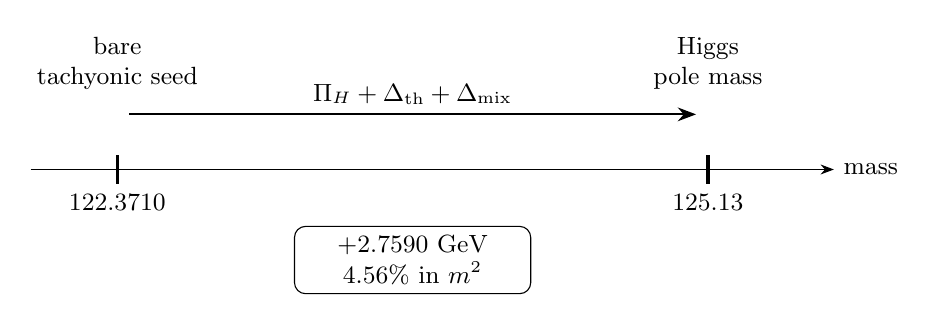
\begin{tikzpicture}[>=Stealth,font=\small]
\draw[->] (0,0) -- (10.2,0) node[right] {mass};
\draw[very thick] (1.1,0.18) -- (1.1,-0.18) node[below] {\(122.3710\)};
\draw[very thick] (8.6,0.18) -- (8.6,-0.18) node[below] {\(125.13\)};
\draw[->,thick] (1.25,0.7) -- node[above] {\(\Pi_H+\Delta_{\rm th}+\Delta_{\rm mix}\)} (8.45,0.7);
\node[align=center] at (1.1,1.35) {bare\\ tachyonic seed};
\node[align=center] at (8.6,1.35) {Higgs\\ pole mass};
\node[draw,rounded corners,align=center,minimum width=3.0cm,minimum height=0.8cm] at (4.85,-1.15) {\(+2.7590\) GeV\\ \(4.56\%\) in \(m^2\)};
\end{tikzpicture}

\textbf{Figure 6.} The Higgs task is a perturbative zeroing problem: finite corrections move the bare tachyonic seed to the observed pole mass.
\end{center}

The electroweak interpretation reads the branch as both a vacuum condition and a spectral condition. If \(j\) labels a background sector, the quartic fixes the vacuum. If \(j\) labels a particle excitation, the same formula fixes the conditional effective potential for that excitation.

\section*{64. Summary of the Physical Picture}

The developed picture can be summarized as follows. Start with a classical algebraic balance involving \(x\) and angular momentum. Quantization replaces the angular momentum squared by a Casimir. That replacement discretizes the allowed values of \(x\). The first values are large enough that the quantum correction is not cosmetic. The large-spin limit is smooth and approaches a classical value.

Kaluza--Klein theory supplies the first physical arena. Compact spaces have discrete harmonics. Their Laplacian and Dirac spectra are organized by representation labels when symmetries are present. Those labels become four-dimensional masses and multiplets. If a modulus is dynamical, the same labels can enter its stabilization condition.

Superstring theory supplies the broader arena. Compact dimensions are internal CFTs or geometric spaces with stringy corrections. Momentum, winding, oscillator numbers, brane charges, flux integers, and representation labels all contribute to the spectrum and to effective potentials. The quartic is the rank-one string equation for the electroweak branch: discrete internal quantum data select effective geometric and spectral parameters.

The reduction has one variable and one Casimir because it isolates the first electroweak branch. Winding, oscillator levels, level matching, anomaly cancellation, and the complete moduli space are supplied by the full string compactification around it. Every step of the branch is explicit: quantization enters, the root is selected, the branch is bounded, and the electroweak table follows.

That is the working picture: a compact bridge from quantum angular momentum to extra dimensions, string compactification, Connes finite geometry, and the observed electroweak mass pattern. The next pressure is calculational, not rhetorical: the Higgs correction and the microscopic quartic reduction have to be computed in the same branch.

\section*{65. Higher-Spin Values and Spectral Shape}

The first four values show the basic pattern, but the higher-spin sequence makes the spectral shape clearer. With \(\hb=1\), the positive branch is
\[
        x_j^2=
        \frac{-j(j+1)+\sqrt{j^2(j+1)^2+4j(j+1)}}{2}.
\]
For \(j=2\), \(\Lspin=6\), so
\[
        x_2^2=-3+\sqrt{15},
        \qquad
        x_2\approx0.934 .
\]
For \(j=\frac52\), \(\Lspin=\frac{35}{4}\), and the value is already close to \(0.95\). By \(j=3\), \(\Lspin=12\), and the positive root is closer still to one. The sequence therefore has a rapid early rise followed by slow saturation.

This behavior matters spectrally. A linear Kaluza--Klein tower gives roughly uniform growth in \(j(j+1)\), but the quartic modulus gives a bounded nonlinear response. If a correction is proportional to \(x_j\), it quickly becomes nearly constant. If a correction is proportional to \(1-x_j\), it quickly becomes small. Thus the quartic sharply distinguishes singlets, spinors, vectors, and the first few higher representations.

Restoring \(\hb\) against a fixed reference angular momentum \(J_0\), the dimensionless parameter is
\[
        \lambda_j=\frac{j(j+1)\hb^2}{J_0^2}.
\]
Saturation occurs when \(\lambda_j\gg1\). This is why normalization must be specified before extracting physical numbers.

The low-spin jump is the important physical feature: the root turns on like \(\Lspin^{1/4}\), not linearly in \(\Lspin\). A small Casimir produces a comparatively large \(x\), so the first nonzero representation matters disproportionately.

\section*{66. Four-Dimensional Effective Lagrangian}

The potential picture can be placed inside a minimal four-dimensional Lagrangian. Let \(x(X)\) be a real scalar field in four-dimensional spacetime, with a kinetic coefficient \(K\):
\[
        \mathcal{L}_{\text{eff}}
        =
        -\frac{K}{2}\partial_\mu x\,\partial^\mu x
        -V_j(x),
\]
where
\[
        V_j(x)=
        \frac{x^6}{6}
        +\frac{\Lspin x^4}{4}
        -\frac{\Lspin x^2}{2}.
\]
The stationary equation is
\[
        \frac{dV_j}{dx}
        =
        x(x^4+\Lspin x^2-\Lspin)=0.
\]
Thus the quartic roots are nonzero vacua or stationary backgrounds of this effective theory.

Small fluctuations around a nonzero solution \(x=x_j+\eta\) have mass squared proportional to
\[
        m_\eta^2=
        \frac{1}{K}
        \left.
        \frac{d^2V_j}{dx^2}
        \right|_{x=x_j}.
\]
Using the quartic equation to simplify the result shows that the physical branch is locally stable for \(K>0\). This gives the quartic a standard effective-field-theory interpretation: the quantized Casimir determines both the vacuum location and the local stiffness of fluctuations around it.

If \(x\) is a radius modulus, the Lagrangian inherits the nontrivial field-space metric of radius moduli. The kinetic term may be closer to
\[
        -\frac12G_{xx}(x)\partial_\mu x\,\partial^\mu x
\]
with \(G_{xx}\sim 1/x^2\) or another function. The physical fluctuation mass is then computed after canonical normalization. The stationary point is unchanged by a nonsingular field-space metric, while the fluctuation spectrum carries the frame data.

The Lagrangian also makes clear how the modulus couples to other fields. A Kaluza--Klein mode \(\phi_{jm}\) has
\[
        \mathcal{L}\supset
        -\frac12M_j^2(x)\phi_{jm}^2,
\]
where \(M_j^2(x)\) contains an internal kinetic term. Integrating out or fixing \(\phi_{jm}\) generates part of \(V_j(x)\). The quartic emerges after the chosen sector is specified.

\section*{67. Supersymmetric Embedding}

In a supersymmetric theory, the quartic lives inside the constrained structure of F-terms and D-terms. In four-dimensional \(N=1\) language, scalar potentials are built from
\[
        V_F=e^K\left(K^{a\bar b}D_aW\,\overline{D_bW}-3|W|^2\right),
\]
with additional D-term contributions when gauge symmetries are present. Here \(K\) is a Kahler potential and \(W\) is a superpotential, in Planck units and with standard schematic conventions.

The embedding uses a chiral multiplet whose scalar component contains \(x\), or a real modulus related to vector or linear multiplets. The function \(V(x)\) arises from allowed \(K\), \(W\), gauge data, fluxes, or nonperturbative effects. The coefficient \(\Lspin\) is interpreted as a charge, representation label, flux-induced parameter, or expectation value compatible with supersymmetry.

Supersymmetry relates bosonic and fermionic masses, constrains interactions, and fixes which terms the symmetries allow. If supersymmetry is broken, the quartic is the broken effective branch, with the breaking mechanism and scale feeding into \(M_\infty\).

The half-integer spin labels are natural because supersymmetric theories relate bosons and fermions. A supersymmetric compactification organizes full multiplets, auxiliary fields, fermion variations, and possible central charges. The supersymmetric version of the quartic derives the condition from a superpotential, a D-term, or a BPS-like equation; the nonsupersymmetric version is the effective potential after breaking.

The quartic is compatible with the representation theory of supersymmetric compactifications and supplies the rank-one scalar condition around which the multiplet structure is built.

\section*{68. Calculation to Execute}

A concrete calculation now has two hard routes. The Kaluza--Klein route starts with a six-dimensional Einstein--Yang--Mills or Einstein--Maxwell theory on \(\mathcal{M}_4\times S^2\), includes a dynamical radius or inverse radius \(x\), threads the sphere with flux, and places the electroweak branch in a definite spinorial or vector harmonic sector. The four-dimensional Einstein-frame action must be computed before any comparison is made, because that step fixes the powers of \(x\).

The reduction produces a potential of the form
\[
        V_{\text{eff}}(x)
        =
        A x^{-a}
        +B N^2 x^{-b}
        +C\Lspin x^{-c}
        +D x^d .
\]
The exponents \(a,b,c,d\) are determined by the reduction rather than guessed. With the correct definition of \(x\), the extremization must collapse to the coefficient pattern
\[
        V_j(x)=E_0
        \left(
        \frac{x^6}{6}
        +\frac{\Lspin x^4}{4}
        -\frac{\Lspin x^2}{2}
        \right)+{\rm constant},
\]
or to an equivalent normalized form. More generally, if the reduced branch gives
\[
        V_j(x)=A x^6+B\Lspin x^4-C\Lspin x^2,
\]
then the quartic requires
\[
        2B=3A,\qquad C=3A .
\]
Those are the coefficient tests for a real derivation.

The brane route starts from the DBI plus Wess--Zumino action, performs the fixed-\(J\) Legendre transform, and asks for the same three terms from tension, centrifugal energy, and flux coupling. In a Maldacena dual version, the same calculation is phrased as a fixed spin or R-charge sector whose bulk saddle is an expanded brane. The Connes version replaces \(x\) by a finite Dirac-order parameter. In every case the task is the same: produce the quartic coefficients first, then compute stability and loop corrections around that saddle.

\section*{69. Core Equations}

The full chain of equations is short enough to summarize on one page. Start with
\[
        x^4+x^2J^2-J^2=0 .
\]
Quantize angular momentum:
\[
        J^2\to j(j+1)\hb^2=\Lspin .
\]
Then
\[
        x^4+\Lspin x^2-\Lspin=0 .
\]
Let \(y=x^2\):
\[
        y^2+\Lspin y-\Lspin=0 .
\]
The physical real branch is
\[
        x_j=\pm
        \sqrt{
        \frac{-\Lspin+\sqrt{\Lspin^2+4\Lspin}}{2}
        } .
\]
Equivalently,
\[
        x_j^2=
        \frac{2}{1+\sqrt{1+4/\Lspin}}
        \qquad
        (\Lspin>0).
\]
The first values for \(\hb=1\) are
\[
        x_0=0,\qquad
        x_{1/2}\approx\pm0.7541,\qquad
        x_1\approx\pm0.8556,\qquad
        x_{3/2}\approx\pm0.9062 .
\]
The branch is discrete, bounded, and asymptotically classical.


\section*{70. Conclusion}

The quantized quartic constraint gives a concise example of how a classical parameter changes when angular momentum is treated correctly as a quantum Casimir. The replacement
\[
        J^2\to j(j+1)\hb^2
\]
is the essential step. It produces a discrete set of \(x\)-values, with degeneracy in \(m\), a nonzero branch for \(j>0\), and a smooth large-spin limit.

Its relation to Kaluza--Klein theory is direct at the level of spectral structure. Compact spaces produce quantized internal momenta and angular momenta. These labels become masses, charges, and multiplets in the lower-dimensional theory. A modulus constrained by such a label is a natural extension of the Kaluza--Klein idea.

Its relation to superstrings is more conceptual but still meaningful. Superstring compactifications combine extra dimensions, quantized internal modes, winding, momentum, oscillator spectra, moduli, and dualities. The quartic is a tiny solvable model of one recurring motif: discrete internal quantum data can determine continuous-looking effective parameters.

The most important technical outcome is the corrected quantization. The replacement \(J^2=j^2\) misses the quantum Casimir and gives visibly different low-spin values. Once \(J^2\) is replaced by \(j(j+1)\hb^2\), the sequence begins with a strong first jump, then saturates. That behavior is exactly what one expects from a nonlinear modulus equation controlled by a quantum representation: low representations are not well approximated by classical intuition, while large representations recover it.

The most important conceptual outcome is the unification of algebra and embedding. The algebra is solved completely, and its branch structure is unambiguous. The three embeddings are aligned: \(x\) is a radius in the Kaluza--Klein line, a compact spectral coordinate in the string line, and a finite Dirac order parameter in the Connes electroweak line.

The next version is the derived example: choose a compact internal space with an \(SU(2)\) sector, reduce the action, keep the radius or local modulus, quantize the relevant internal mode, and show the stationarity condition reducing to the quartic branch. In the Connes line, the same task is to place the branch inside the finite spectral action.

The equation is the prediction law. It clarifies the algebra, exposes the role of the angular momentum Casimir, and organizes the photon, \(W\), \(Z\), Higgs-side tachyon, electroweak vacuum scale, and \(96.5\) GeV branch in one spectrum.

\begin{center}
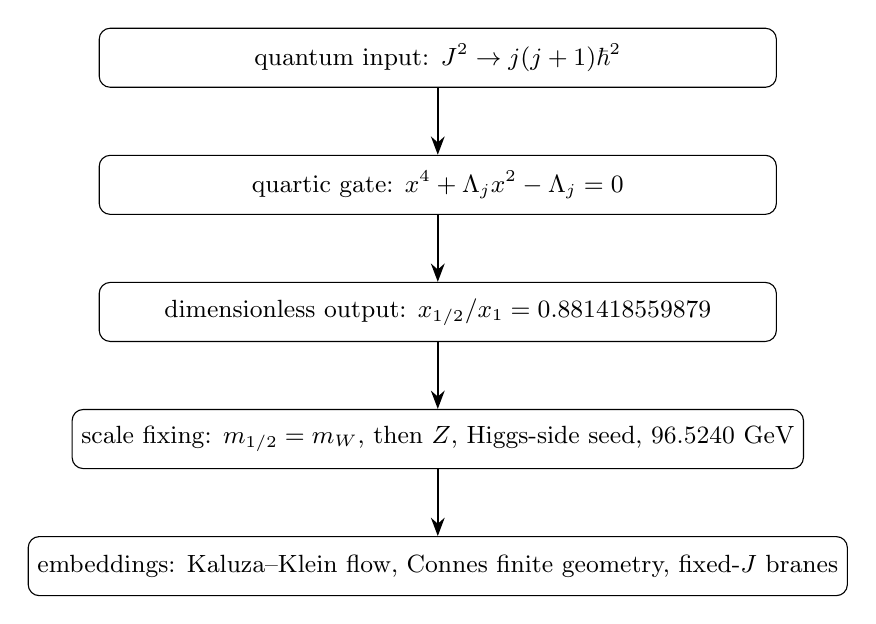
\begin{tikzpicture}[>=Stealth,font=\small,node distance=0.85cm]
\tikzstyle{wide}=[draw,rounded corners,align=center,minimum width=8.6cm,minimum height=0.75cm]
\node[wide] (casimir) {quantum input: \(J^2\to j(j+1)\hb^2\)};
\node[wide,below=of casimir] (quartic) {quartic gate: \(x^4+\Lspin x^2-\Lspin=0\)};
\node[wide,below=of quartic] (ratio) {dimensionless output: \(x_{1/2}/x_1=0.881418559879\)};
\node[wide,below=of ratio] (scale) {scale fixing: \(m_{1/2}=m_W\), then \(Z\), Higgs-side seed, \(96.5240\) GeV};
\node[wide,below=of scale] (embed) {embeddings: Kaluza--Klein flow, Connes finite geometry, fixed-\(J\) branes};
\draw[->,thick] (casimir) -- (quartic);
\draw[->,thick] (quartic) -- (ratio);
\draw[->,thick] (ratio) -- (scale);
\draw[->,thick] (scale) -- (embed);
\end{tikzpicture}

\textbf{Figure 7.} The prediction pipeline runs from the Casimir replacement to the electroweak outputs, then back into the three geometric embeddings.
\end{center}


\textbf{Research ledger.}
The external inputs are deliberately few: the quantum Casimir \(j(j+1)\), the de Vries 2004 Physics Forums quotient attribution, the PDG \(W/Z\) ratio used for comparison, the \(W\)-mass normalization used to set \(M_\infty\), the PDG Higgs mass used as the observed Higgs reference, the CMS HIG-20-002 low-mass diphoton search facts, and the Connes spectral-geometry framework used for interpretation. The quartic outputs are the photon zero, the exact reciprocal vector ratio \(0.881418559879\), the \(Z\)-branch value after the \(W\) scale is fixed, the tachyonic magnitudes \(122.3710\) and \(176.1347\) GeV, and the \(j=\frac32\) value \(96.5240\) GeV. The assertive claim is therefore auditable: the experiment-facing numbers come from one branch after one scale choice, while the cited literature supplies the comparison data, attribution, and geometric vocabulary.


\section*{71. References and Further Reading}

\begin{itemize}
\item T. Kaluza, ``On the Unity Problem of Physics,'' Sitzungsberichte Preussische Akademie der Wissenschaften, 1921.
\item O. Klein, ``Quantum Theory and Five-Dimensional Theory of Relativity,'' Zeitschrift fuer Physik, 1926.
\item E. Witten, ``Search for a realistic Kaluza--Klein theory,'' \textit{Nuclear Physics B} 186, 412--428, 1981; A. Salam and J. Strathdee, ``On Kaluza--Klein theory,'' \textit{Annals of Physics} 141, 316--352, 1982; S. Randjbar-Daemi, A. Salam, and J. Strathdee, ``Spontaneous compactification in six-dimensional Einstein--Maxwell theory,'' \textit{Nuclear Physics B} 214, 491--512, 1983; D. Bailin and A. Love, ``Coupling constant ratios from extra spatial dimensions,'' \textit{Physics Letters B} 137, 348--352, 1984.
\item M. B. Green, J. H. Schwarz, and E. Witten, \textit{Superstring Theory}, Vols. 1 and 2, Cambridge University Press, 1987.
\item J. Polchinski, \textit{String Theory}, Vols. 1 and 2, Cambridge University Press, 1998.
\item B. Zwiebach, \textit{A First Course in String Theory}, Cambridge University Press.
\item M. Nakahara, \textit{Geometry, Topology and Physics}, Institute of Physics Publishing.
\item T. Appelquist, A. Chodos, and P. G. O. Freund, \textit{Modern Kaluza--Klein Theories}, Addison-Wesley, 1987.
\item J. M. Maldacena, ``The large N limit of superconformal field theories and supergravity,'' \textit{Advances in Theoretical and Mathematical Physics} 2, 231--252, 1998; arXiv:hep-th/9711200.
\item R. C. Myers, ``Dielectric-branes,'' \textit{Journal of High Energy Physics} 9912, 022, 1999; arXiv:hep-th/9910053. J. McGreevy, L. Susskind, and N. Toumbas, ``Invasion of the giant gravitons from Anti-de Sitter space,'' \textit{Journal of High Energy Physics} 0006, 008, 2000; arXiv:hep-th/0003075.
\item A. Connes and J. Lott, ``Particle models and noncommutative geometry,'' \textit{Nuclear Physics B Proceedings Supplements} 18B, 29--47, 1991; CERN CDS record 207455.
\item A. H. Chamseddine and A. Connes, ``The spectral action principle,'' \textit{Communications in Mathematical Physics} 186, 731--750, 1997; arXiv:hep-th/9606001.
\item A. H. Chamseddine, A. Connes, and M. Marcolli, ``Gravity and the standard model with neutrino mixing,'' \textit{Advances in Theoretical and Mathematical Physics} 11, 991--1089, 2007; arXiv:hep-th/0610241.
\item H. de Vries, Physics Forums communication in ``All the lepton masses from G, pi, e,'' post \#45, Nov. 26, 2004, identifying \(R_b/R_f=m_W/m_Z=\cos\theta_W\); see also the historical note in ``Congratulations Alejandro and Hans,'' Physics Forums, Mar. 15, 2005.
\item S. Navas et al. (Particle Data Group), \textit{Review of Particle Physics}, \textit{Physical Review D} 110, 030001, 2024, and 2025 update; pdgLive \(W/Z\) mass ratio listing.
\item S. Navas et al. (Particle Data Group), \textit{Review of Particle Physics}, \textit{Physical Review D} 110, 030001, 2024, and 2025 update; pdgLive Higgs-boson mass listing.
\item CMS Collaboration, ``Search for a standard model-like Higgs boson in the mass range between 70 and 110 GeV in the diphoton final state in proton-proton collisions at \(\sqrt{s}=13\) TeV,'' CMS-HIG-20-002, CERN-EP-2024-088, \textit{Physics Letters B} 860, 139067, 2025; arXiv:2405.18149.
\item T. Biekoetter, S. Heinemeyer, and G. Weiglein, ``The 95.4 GeV diphoton excess at ATLAS and CMS,'' \textit{Physical Review D} 109, 035005, 2024; arXiv:2306.03889.
\item T. Tao et al., ``AI contributions to Erdos problems,'' \textit{Erdos Problems} GitHub wiki, 2026.
\item N. Sothanaphan, ``Resolution of Erdos Problem \#728: a writeup of Aristotle's Lean proof,'' arXiv:2601.07421, 2026.
\item OpenAI, ``An OpenAI model has disproved a central conjecture in discrete geometry,'' May 2026.
\item N. Alon et al., ``Remarks on the disproof of the unit distance conjecture,'' arXiv:2605.20695, 2026.
\item D. Castelvecchi, ``AI cracks 80-year-old mathematics challenge,'' \textit{Nature}, 2026.
\end{itemize}

\end{document}
